\chapter{Mejoras a WebSim}
\label{chap:mejoras}
Una vez presentado el contexto, objetivos y herramientas empleadas, en este capitulo se detallan todas las mejoras realizadas del simulador \textit{WebSim} y cómo se han llevado a cabo. Se va a explicar cómo se han integrado los \textit{drones} ampliando los drivers existentes para incluir nueva funcionalidad, el modelo en 3D o los bloques de \textit{Scratch} necesarios, los teleoperadores desarrollados y sus ficheros de configuración. También se detallan los nuevos ejercicios creados, tanto individuales como competitivos, que incorporan evaluadores automáticos para puntuar el funcionamiento de los \textit{robots} programados.

\section{Soporte a drones y nuevos robots}
\label{sec:drone}

Uno de los objetivos principales del TFG era ampliar el soporte para otros robots y escenarios en \textit{WebSim}. Se ha comenzado dando soporte a drones debido a las diferencias con el \textit{robot PiBot} del que ya disponía soporte. 
Para ello hay que extender el \textit{software} existente de la plataforma.
\subsection{Driver del drone e interfaz de programación en \textit{JavaScript}}

Una de las principales diferencias entre el \textit{drone} y el robot con ruedas \textit{PiBot} es el movimiento vertical o en el eje Y (en la figura \ref{fig:ejesFrame} se puede ver una representación del sistema de coordenadas de \textit{A-Frame}) tanto para darle velocidad al \textit{drone} como para actualizar la posición. 

\begin{figure}[H]
    \centering
    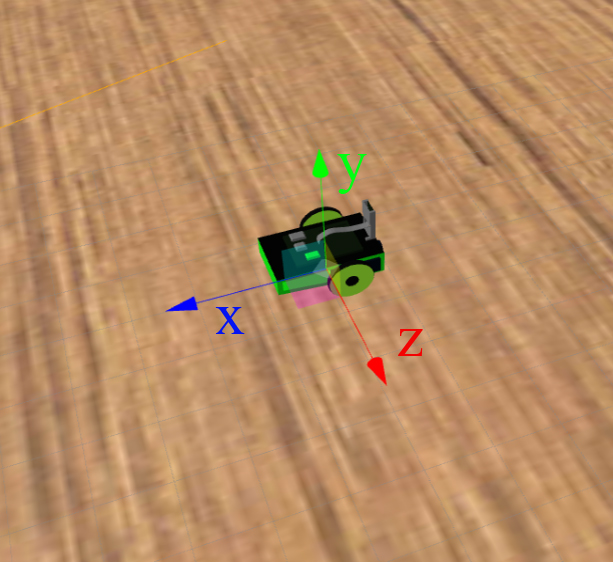
\includegraphics[scale=0.3]{img/ejesframe.jpg}
    \caption{Sistema de ejes en A-Frame} \label{fig:ejesFrame}
\end{figure}

Se han creado las siguiente funciones para ello:
\begin{itemize}
    \item \textit{\textbf{setL()}}: Método que permite ordenar velocidad vertical al \textit{robot}. 
    
    \begin{lstlisting}[language=javascript]
    setL(l){
        this.velocity.y = l;
    }
    \end{lstlisting}
    
    \item \textit{\textbf{getL()}}: Método que devuelve la velocidad vertical del \textit{robot}.
    
    \begin{lstlisting}[language=javascript]
getL(){
    return this.velocity.y;
}
    \end{lstlisting}
    
    \item \textit{\textit{\textbf{despegar()}}}: Método que imprime velocidad vertical al \textit{robot} hasta alcanzar cierta altura.
    
    \begin{lstlisting}[language=javascript]
    despegar(){
        this.velocity.y=3; 
        await sleep(0.5);
        this.velocity.y=0;
    }
    \end{lstlisting}
    
    \item \textit{\textbf{aterrizar()}}: Método que imprime velocidad vertical negativa al \textit{robot} hasta que alcance el suelo.
    
    \begin{lstlisting}[language=javascript]
    aterrizar(){
        this.velocity.y=-3;
        await sleep(0.4);
        this.velocity.y=0;
    }
    \end{lstlisting}
    
\end{itemize}

Además, se han editado funciones y variables que ya existían para ampliar su funcionalidad: 
\begin{itemize}
    \item \textit{\textbf{move()}}: ahora acepta 3 parámetros y se incluye  velocidad vertical como nuevo:
        \begin{lstlisting}[language=javascript]
            move(v, w, h){
                this.setV(v);
                this.setW(w);
                this.setL(h);
            }
        \end{lstlisting}
    \item \textit{\textbf{updatePosition()}}: se ha extendido para poder actualizar el eje Y para representarlo en la escena de \textit{A-Frame}:
    \begin{lstlisting}[language=javascript]
    updatePosition(rotation, velocity, robotPos){
      let x = velocity.x/10 * Math.cos(rotation.y * Math.PI/180);
      let z = velocity.x/10 * Math.sin(-rotation.y * Math.PI/180);
      let y = (velocity.y/10);
      robotPos.x += x;
      robotPos.z += z;
      robotPos.y += y;
      return robotPos;
    }
\end{lstlisting}
    \item \textit{\textbf{this.velocity}}: se ha ampliado la variable de la clase \textit{robot} que guarda la velocidad:
    
\begin{lstlisting}[language=javascript]
        this.velocity = {x:0, y:0, z:0, ax:0, ay:0, az:0};
\end{lstlisting}
\end{itemize}


En la tabla \ref{tab:tablaMotores2} se recopilan todas las funciones del \textit{HAL API} que extienden la plataforma para dar soporte a \textit{drones}.

\begin{table}[H]
  \begin{center}
    \caption{Métodos (HAL API) de los actuadores implementados para el drone.}
    \vspace{0.5cm}
    \label{tab:tablaMotores2}
    \begin{tabular}{|c|c|} 
    \hline
      \textbf{Método} & \textbf{Descripción}\\
      \hline
.setL(integer) & \begin{tabular}[c]{@{}c@{}}Mueve a cierta velocidad hacia arriba o hacia abajo el robot.\\\end{tabular} \\ \hline
.getL() & \begin{tabular}[c]{@{}c@{}}Devuelve la velocidad vertical del robot.\\\end{tabular} \\ \hline
.move(integer, integer, integer) & \begin{tabular}[c]{@{}c@{}}Mueve el robot a ciertas velocidades hacia delante/atrás,\\ arriba/abajo y gira al mismo tiempo.\\ \end{tabular} \\ \hline
.despegar() & \begin{tabular}[c]{@{}c@{}}Comanda velocidad vertical al robot hasta que \\ alcanza una determinada altura.\\ \end{tabular} \\ \hline
.aterrizar() & \begin{tabular}[c]{@{}c@{}}Comanda velocidad vertical negativa al robot hasta que \\ alcanza el suelo.\\ \end{tabular} \\ \hline
    \end{tabular}
  \end{center}
\end{table}

Uno de los principales problemas encontrados es que el motor de físicas de \textit{A-Frame} no simula correctamente la posición de robot al otorgarle velocidad vertical y hace que el robot ``rebote'' sobre el escenario. Esto es debido a que el escenario tiene un atributo llamado ``gravedad'' que se aplica cada pocos milisegundos y entra en conflicto con la función \textit{updatePosition}. Se ha solucionado cambiando su valor haciendo que el escenario carezca de gravedad cuando se simula el \textit{drone}. 

\subsection{Modelo 3D, apariencia}

Para simular el robot en el entorno de \textit{A-Frame} es necesario realizar un modelo tridimensional. Para ello se ha buscado un modelo disponible en un repositorio\cite{bib:sketchfab} y se ha retocado en \textit{Blender} (figura \ref{fig:droneBlender}) para que se ajuste a los requisitos del entorno. Las modificaciones que se han realizado al modelo son: 
\begin{itemize}
    \item Reducción de polinomios (modelo \textit{low-poly}) para disminuir el peso del modelo y aliviar los tiempos de carga del escenario.
    \item Rotación del modelo para que encaje con la orientación que disponía el anterior robot. Es decir, que el robot tenga su parte frontal mirando hacia el eje X positivo para que al comandarle velocidad lineal se desplace hacia delante.
    \item El modelo 3D dispone de focos de luz, que son independientes de la luz que proporciona \textit{A-Frame}. Se ha suprimido o desplazado para adaptarla al escenario.
    
    \item Elaborar una animación a las hélices para darle un aspecto más realista usando animaciones de \textit{A-Frame}, que se activa vía \textit{software} cuando el drone despega del suelo.
    
\end{itemize}

 \begin{figure}[H]
    \centering
    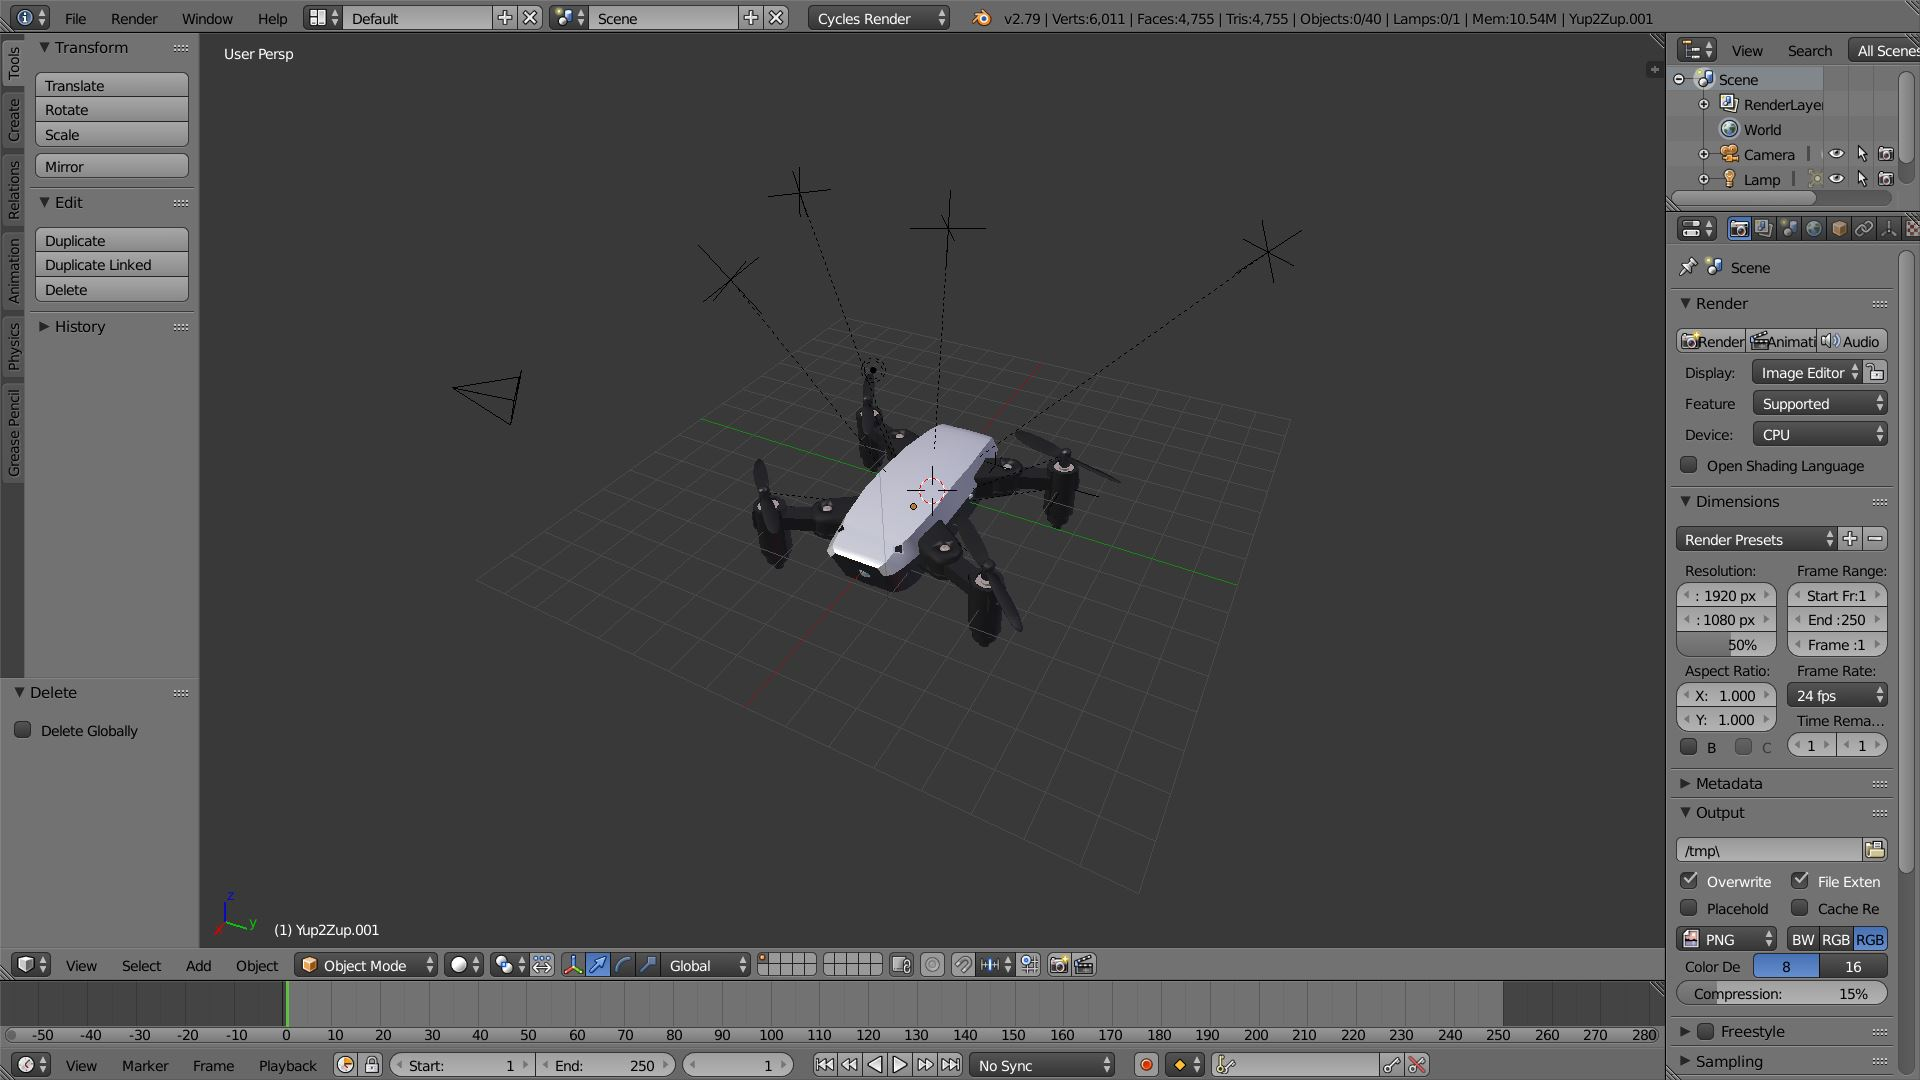
\includegraphics[scale=0.3]{img/droneBlender.jpg}
    \caption{Drone en Blender} \label{fig:droneBlender}
\end{figure}


\textit{Blender} genera un fichero \textit{gltf} y da la posibilidad de contener en él un binario que incluye las animaciones o exportarlo en dos distintos. En este caso, se ha hecho como un único fichero y tiene un aspecto similar al formato \textit{JSON}\footnote{\url{https://github.com/RoboticsLabURJC/2019-tfg-ruben-alvarez/blob/master/upgrades/drones/drone_animation.gltf}}. 

El drone implementado en el entorno de \textit{WebSim} se puede ver en la figura \ref{fig:escenarioDrone}.

   \begin{figure}[H]
    \centering
    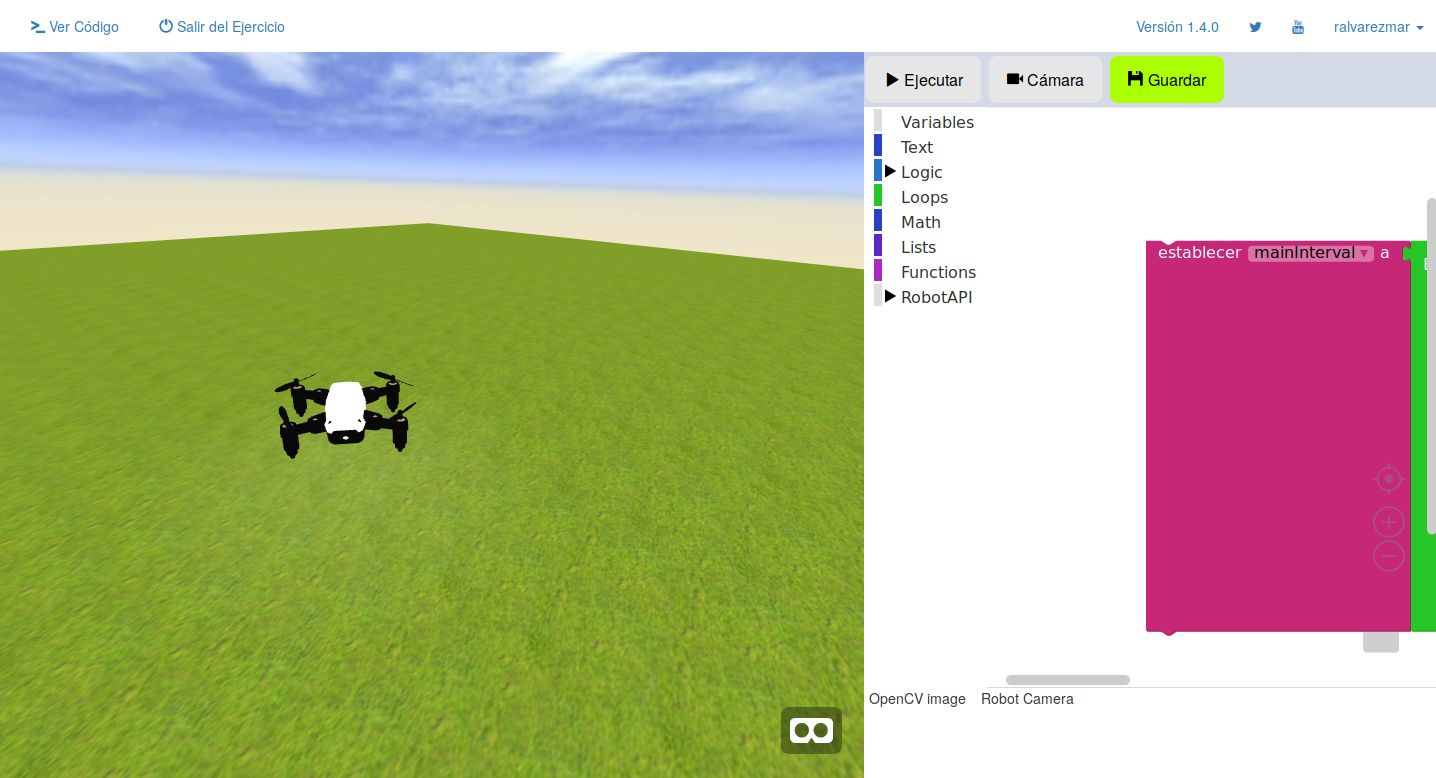
\includegraphics[scale=0.3]{img/websimDrone.png}
    \caption{Escenario de WebSim con drone integrado} \label{fig:escenarioDrone}
    \end{figure}

También se han creado modelos de \textit{drones} de distintos colores para su disposición en ejercicios que requieran más de un \textit{robot} en el escenario: 

      \begin{figure}[H]
        \centering
        \begin{subfigure}{0.3\textwidth}
         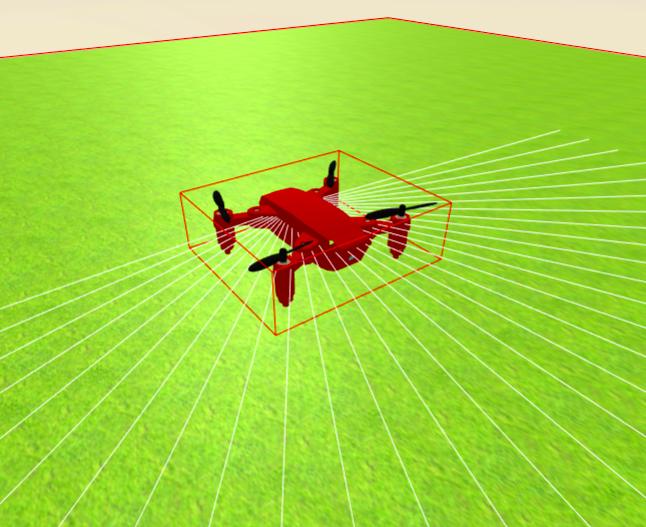
\includegraphics[width=4cm, height=3cm]{img/red_drone.png}
 \label{fig:drone_rojo}
        \end{subfigure}
        \begin{subfigure}{0.3\textwidth}
         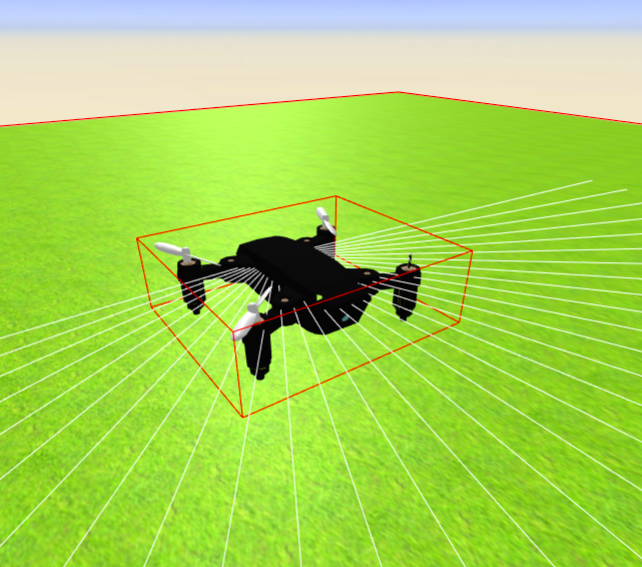
\includegraphics[width=4cm, height=3cm]{img/black_drone.png}
   \label{fig:drone_negro}
        \end{subfigure}
        \begin{subfigure}{0.3\textwidth}
         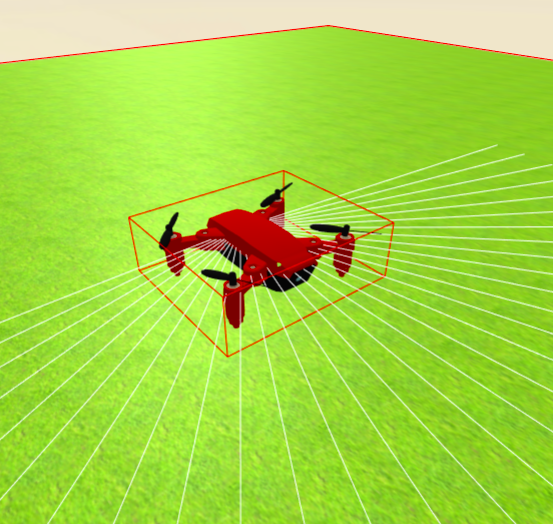
\includegraphics[width=4cm, height=3cm]{img/red_blackdrone.png}
   \label{fig:drone_negrorojo}
        \end{subfigure}
          \caption{Modelos de \textit{drone} de distintos colores}
    \end{figure}

\subsection{Bloques Scratch para programación gráfica del drone}
\label{subsec:bloques}
Una vez implementado el código \textit{JavaScript} para el soporte del drone, es necesario crear los bloques con \textit{Blockly} para añadir sus funcionalidad en el editor de \textit{Scratch}. 

Para ello, se han creado 4 bloques con las funciones anteriormente explicadas: 
\begin{itemize}
    \item Velocidad ascenso: Comanda la velocidad ascendente del bloque que se le adjunte. 
    \begin{figure}[H]
        \centering
        
\includegraphics[width=0.3\textwidth]{img/ascensionBlockly.png}
        \caption{Bloque de velocidad de ascenso} \label{fig:ascension}
    \end{figure}
    
    \item Velocidad descenso: Comanda al robot la velocidad descendente del bloque que se le adjunte. 
    \begin{figure}[H]
        \centering
        
\includegraphics[width=0.3\textwidth]{img/descensoBlockly.png}
        \caption{Bloque de velocidad de descenso} \label{fig:descenso}
    \end{figure}
    \item Aterrizar: Comanda velocidad vertical negativa al \textit{drone} hasta que alcance el suelo. Mantendrá esa posición hasta recibir una nueva orden.
    \begin{figure}[H]
        \centering
        
\includegraphics[width=0.2\textwidth]{img/aterrizarBlockly.png}
        \caption{Bloque de aterrizaje} \label{fig:aterrizaje}
    \end{figure}
    \item Despegar: Comanda velocidad vertical positiva al \textit{drone} hasta que alcance cierta altitud. 
        \begin{figure}[H]
            \centering
            
\includegraphics[width=0.2\textwidth]{img/despegarBlockly.png}
            \caption{Bloque de despegue} \label{fig:despegar}
        \end{figure}
\end{itemize}

 Como ejemplo ilustrativo se muestra en detalle la traducción del bloque despegar, que va incluida (junto a los otros bloques creados) en el directorio de bloques personalizados.

\begin{lstlisting}[language=javascript,label=lst:tradAterrizar,basicstyle=\tiny]
export default function initLandBlock(){
  var landBlock = {
  "type": "land",
  "message0": "Despegar %1",
  "args0": [
    {
      "type": "field_variable",
      "name": "NAME",
      "variable": "MyRobot"
    }
  ],
  "previousStatement": null,
  "nextStatement": "String",
  "colour": "%{BKY_MATH_HUE}",
  "tooltip": "Aterriza el drone",
  "helpUrl": "Aterriza el drone"
}
  Blockly.Blocks['land'] = {
    init: function() {
      this.jsonInit(landBlock);
    }
  };
  Blockly.JavaScript['land'] = function(block) {
    var variable_name = Blockly.JavaScript.variableDB_.getName(block.getFieldValue('NAME'), Blockly.Variables.NAME_TYPE);
    var value_robotvar = Blockly.JavaScript.valueToCode(block, 'ROBOTVAR', Blockly.JavaScript.ORDER_ATOMIC);
    var code = variable_name + '.aterrizar(); \n';
    return code;
  };
  Blockly.Python['land'] = function(block) {
    var variable_name = Blockly.Python.variableDB_.getName(block.getFieldValue('NAME'), Blockly.Variables.NAME_TYPE);
    var value_robotvar = Blockly.Python.valueToCode(block, 'ROBOTVAR', Blockly.Python.ORDER_ATOMIC);
    var code = variable_name + '.aterrizar()\r\n';
    return code;
  };
}
\end{lstlisting}

Para que los bloques aparezcan en el editor de \textit{Scratch} es necesario importarlos e inicializarlos en el fichero que lo configura. En la siguiente imagen se muestra el espacio de trabajo de \textit{Scratch} con los nuevos bloques incorporados:

\begin{figure}[H]
    \centering            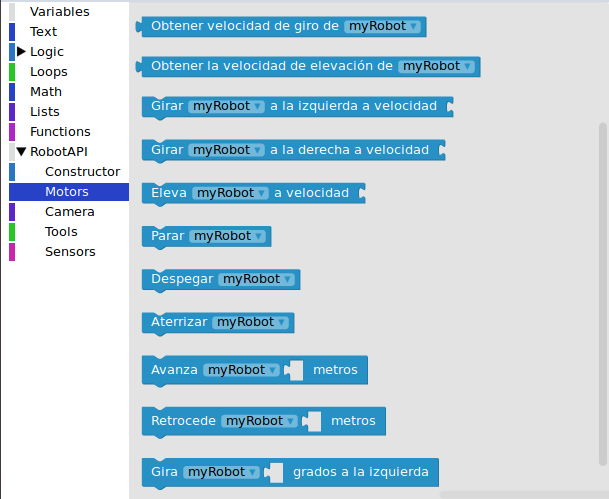
\includegraphics[width=0.65\textwidth]{img/kibotics_newblocks.png}
    \caption{Espacio de trabajo de \textit{Scratch} con los bloques del drone incorporados} 
    \label{fig:newblocks}
\end{figure}

\subsection{Nuevos robots}
\label{subsec:nuevosrobots}

Además del soporte a \textit{drones}, se han incluido nuevos \textit{robots} a \textit{WebSim}: 

\begin{itemize}
    \item \textbf{Fórmula 1}: se han creado dos modelos distintos para incorporarlos a ejercicios que necesiten dos robots en la misma escena y que haya diferencias entre ambos para poder distinguirlos. 
    
      \begin{figure}[H]
        \centering
        \begin{subfigure}{0.4\textwidth}
         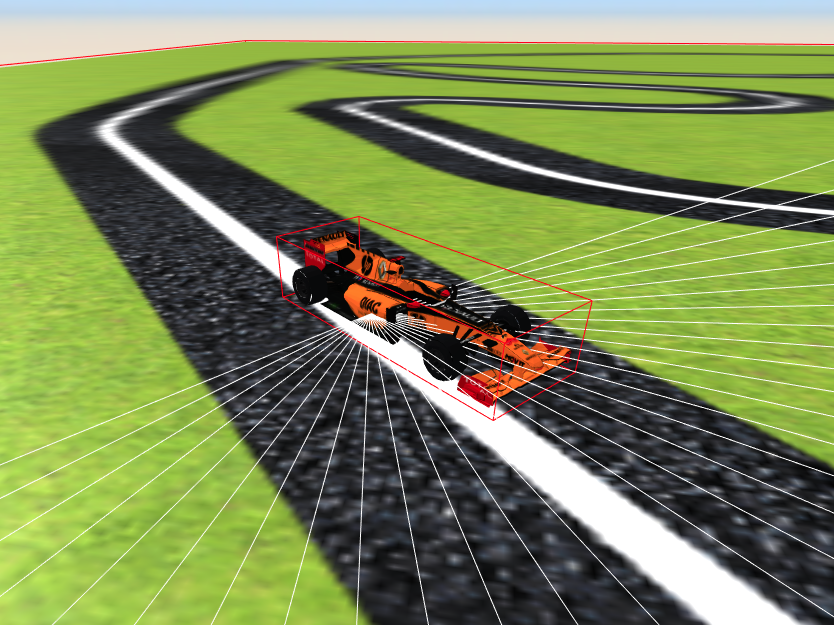
\includegraphics[width=6cm, height=5cm]{img/f1_renault.png}
 \label{fig:f1_renault}
        \end{subfigure}
        \begin{subfigure}{0.4\textwidth}
         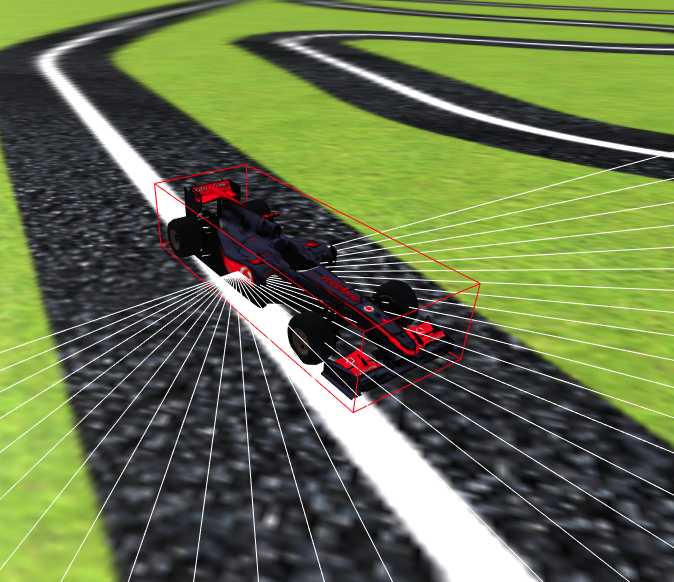
\includegraphics[width=6cm, height=5cm]{img/f1_williams.png}
   \label{fig:f1_williams}
        \end{subfigure}
          \caption{Modelos de coches Fórmula 1}
    \end{figure}

  \item \textbf{mBot}: creado por la disponibilidad del \textit{robot} real y su facilidad para añadir elementos al \textit{robot} en la simulación.
    \begin{figure}[H]
    \centering            
    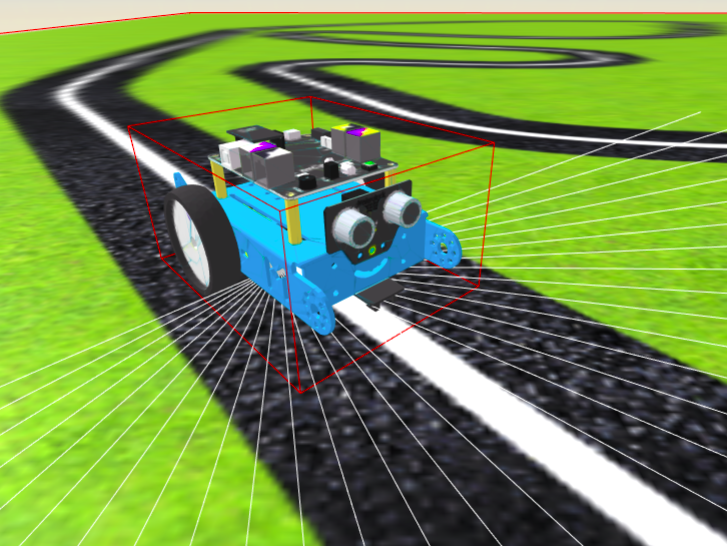
\includegraphics[scale=0.25]{img/mBot_model.png}
    \caption{Modelo mBot} \label{fig:mBot}
    \end{figure}
    
\end{itemize}

\section{Teleoperadores en WebSim}
\label{sec:teleoperadores}

Se han incorporado teleoperadores en \textit{WebSim} para poder controlar los robots sin necesidad de programarlos. De esta manera es posible saber el estado y valor de sus sensores de manera sencilla ayudando a los desarrolladores a buscar fallos en drivers o incorporar nuevos escenarios. 
Su principal utilidad es ayudar a depurar la implementación de los nuevos \textit{robots} desarrollados, el correcto funcionamiento de sus actuadores, sus sensores y sus interfaces de programación. 

\subsection{Interfaz gráfica}

Se han creado teleoperadores para los modelos del \textit{piBot}, \textit{mBot}, \textit{Formula 1} y del \textit{drone}. Los 3 primeros tienen la misma interfaz gráfica y el último incorpora dos botones para controlar la velocidad vertical. 


\begin{figure}[H]
\centering
\begin{subfigure}[b]{0.475\textwidth}
\centering
    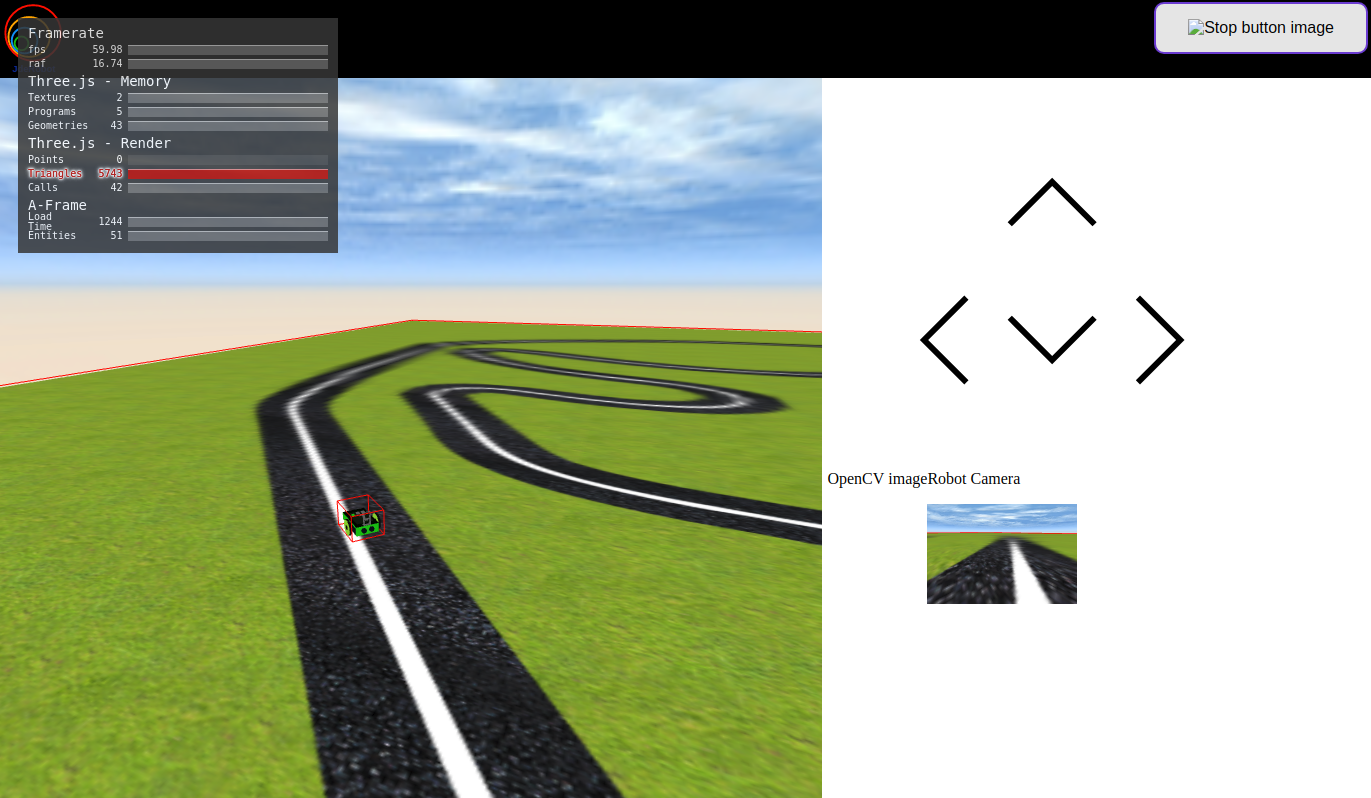
\includegraphics[width=\textwidth]{img/pibot_teleoperator.png}
\label{fig:pibottele}
\end{subfigure}
\hfill
\begin{subfigure}[b]{0.475\textwidth}\centering

  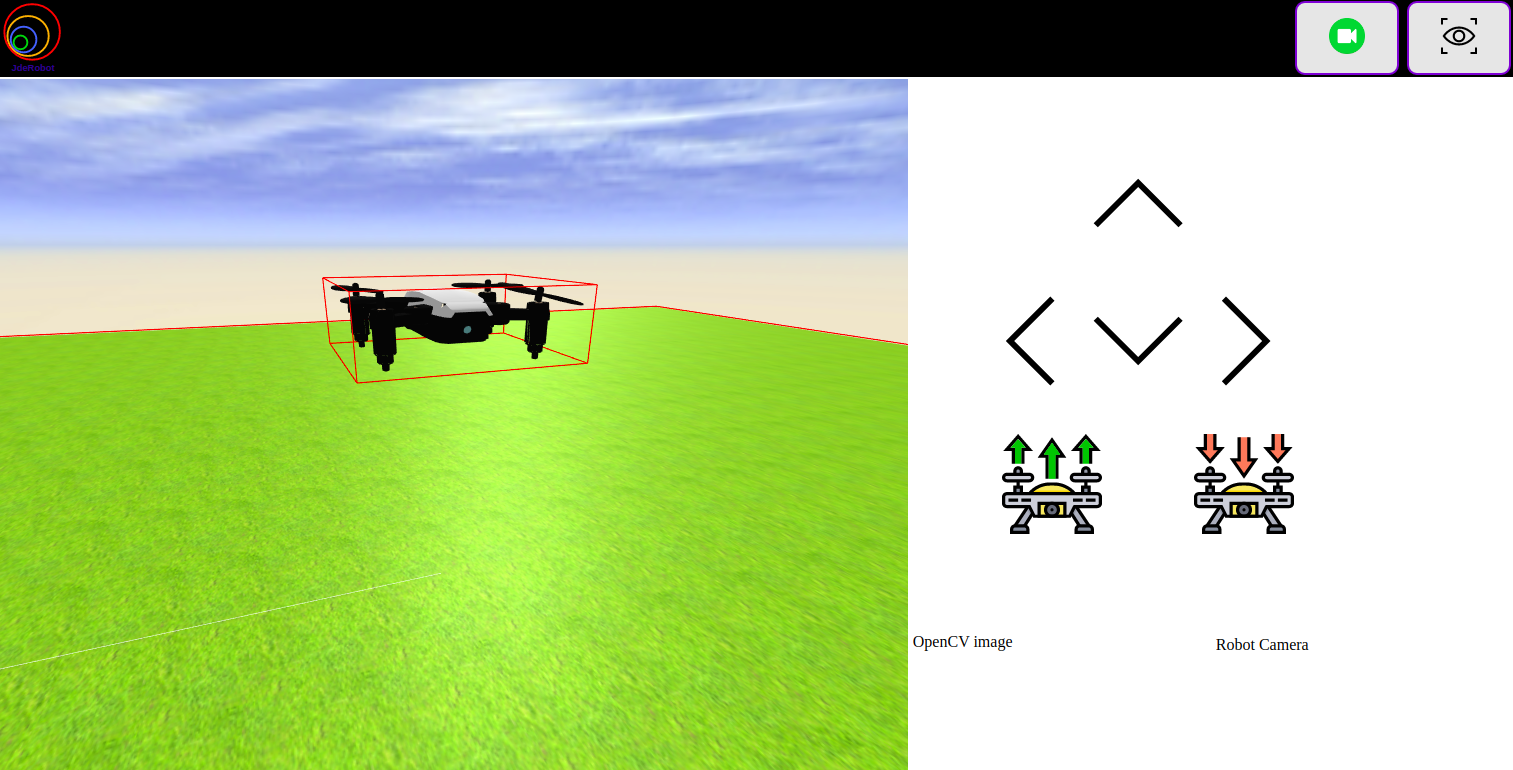
\includegraphics[width=\textwidth]{img/drone_teleoperator.png}
\label{fig:dronetele}
\end{subfigure} 
\vskip\baselineskip
\begin{subfigure}[b]{0.475\textwidth}
\centering
    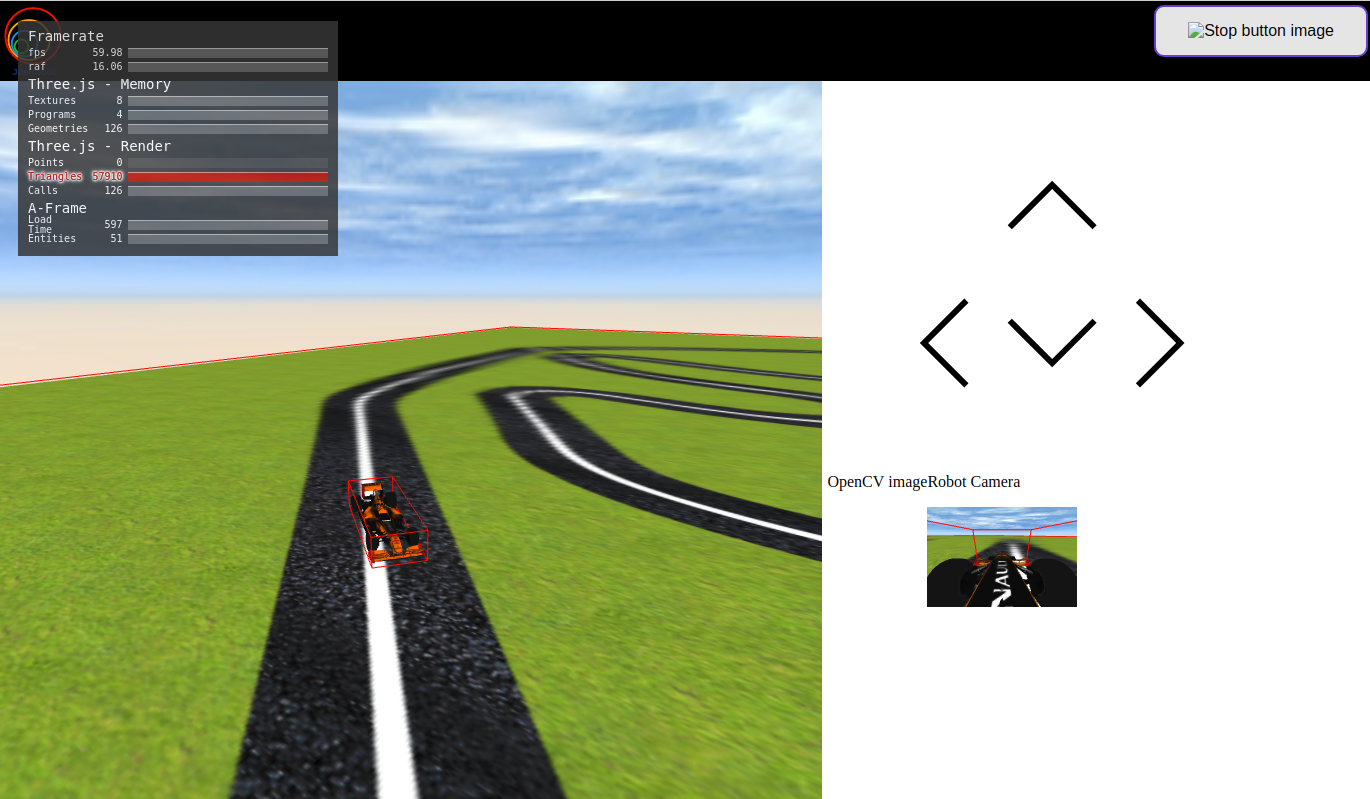
\includegraphics[width=\textwidth]{img/f1_teleoperator.png}
\label{fig:f1tele}
\end{subfigure}
\hfill
\begin{subfigure}[b]{0.475\textwidth}
\centering
    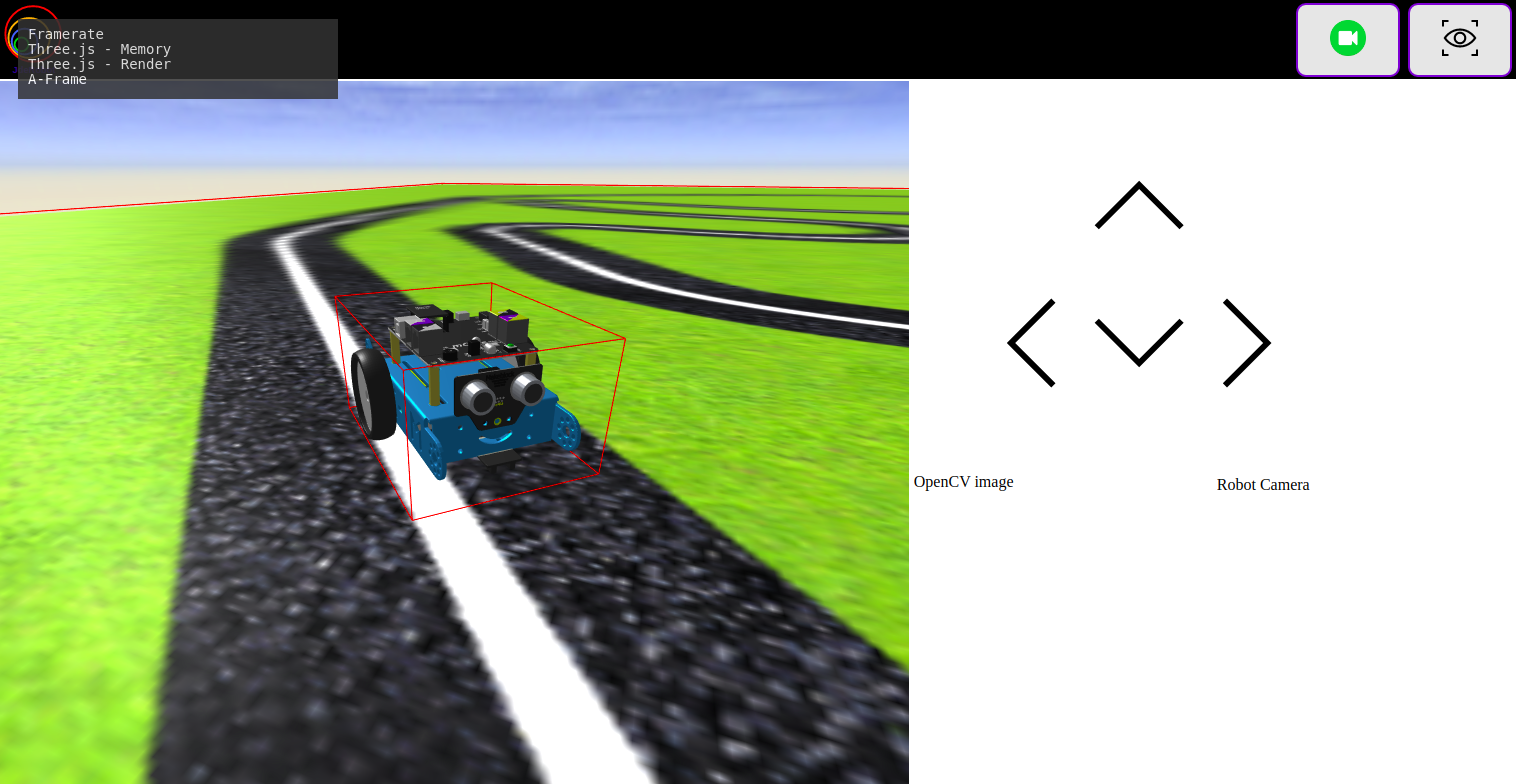
\includegraphics[width=\textwidth]{img/mBot_teleoperator.png}
\label{fig:mbotele}
\end{subfigure}
\label{fig:teleoperadores}
\end{figure}

Siendo el código fuente \textit{HTML} empleado para el teleoperador del drone el mostrado a continuación: 

\begin{lstlisting}[language=html,label=lst:teleop,caption=Código HTML del teleoperador del drone]
<div id="right-container">
<div class="buttons">
  <div id="upArrow">
      <button onclick class="buttonArrow" id="invisible"><img class="buttonArrow" src="../assets/resources/speed.svg" /></button>
      <button onclick class="buttonArrow" id="speed"><img class="buttonArrow" src="../assets/resources/speed.svg" /></button>
  </div>
  <div id="bottomArrows">
      <button onclick class="buttonArrow" id="left" ><img class="buttonArrow" src="../assets/resources/left.svg"/></button>
      <button onclick class="buttonArrow" id="brake"><img class="buttonArrow" src="../assets/resources/brake.svg"/></button>
      <button onclick class="buttonArrow" id="right"><img class="buttonArrow" src="../assets/resources/right.svg"/></button><br>
  </div>
  <div id="takeoff">
    <button onclick id="up"><img class="buttonArrow" src="../assets/resources/goUp.svg" /></button>
    <button onclick id="down"><img class="buttonArrow" src="../assets/resources/goDown.svg" /></button></button>
  </div>
</div>
\end{lstlisting}

También se ha creado una página \textit{web}  única para acceder a todos ellos: 

 \begin{figure}[H]
    \centering
    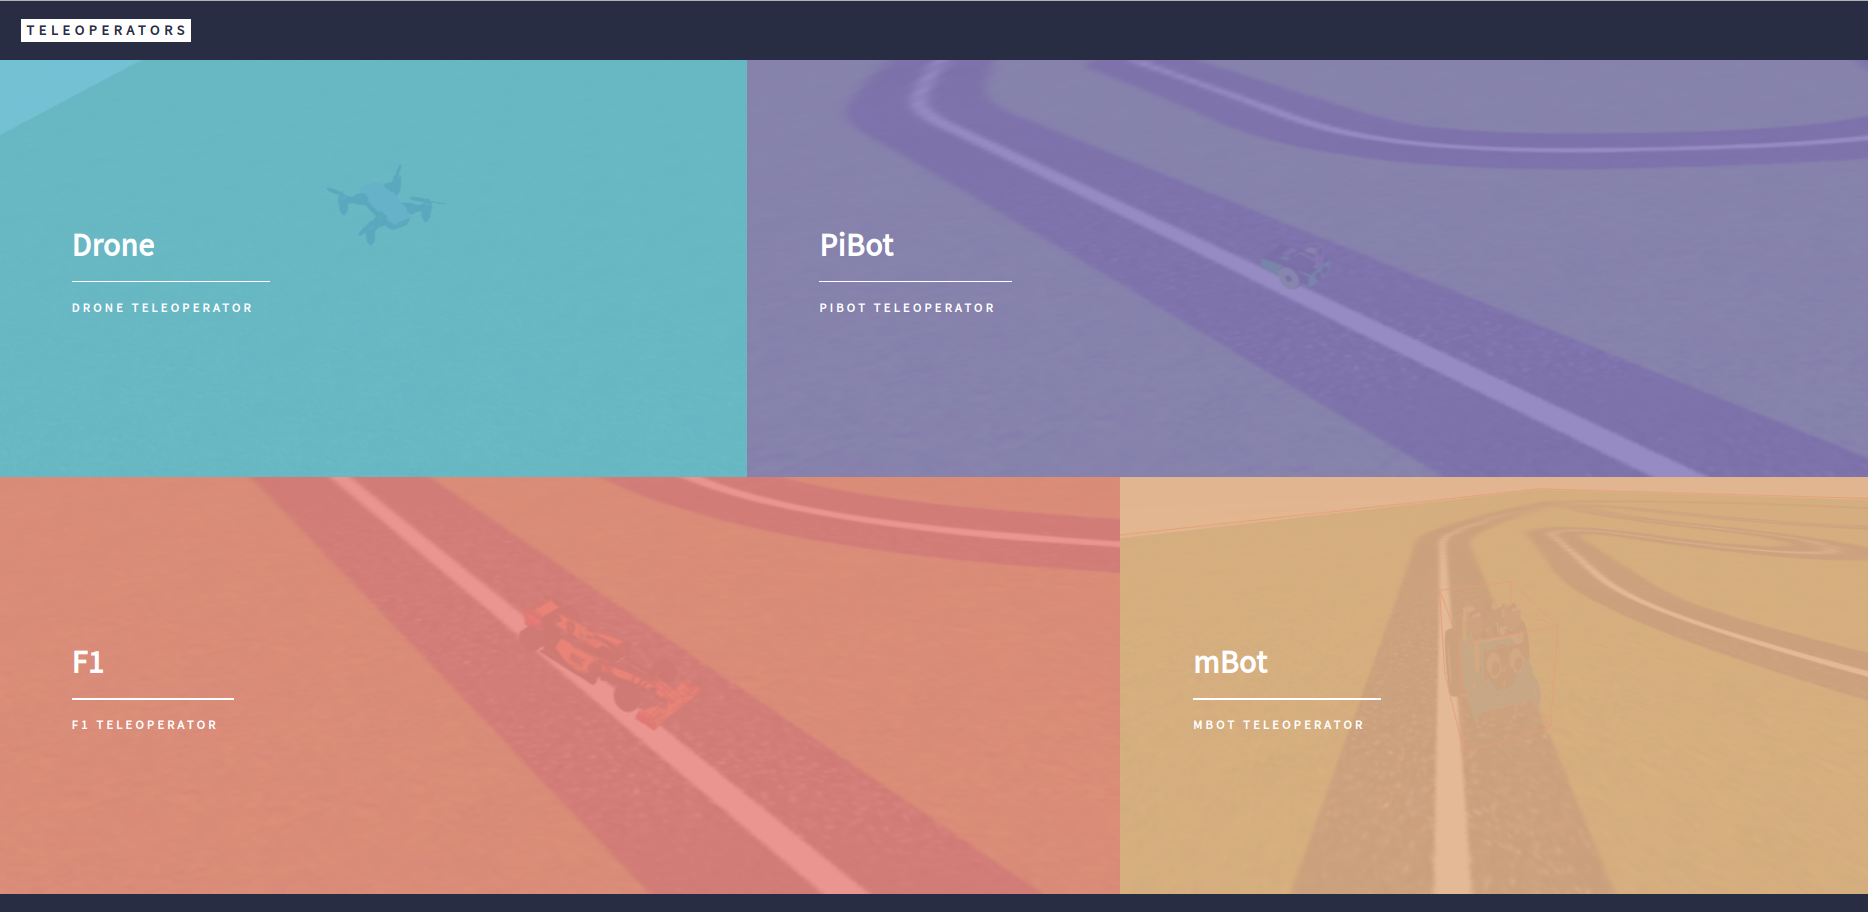
\includegraphics[scale=0.25]{img/teleoperators.png}
    \caption{Interfaz que permite acceder a cada uno de los teleoperadores} \label{fig:teleoperators}
\end{figure}

\begin{lstlisting}[language=html,label=lst:teleopMain,caption=Código HTML de la interfaz para acceder a los teleoperadores]
<body>
   <div id="wrapper">
      <header id="header" class="alt">
         <p class="logo"><strong>Teleoperators</strong></a>
      </header>
      <div id="main">
         <section id="one" class="tiles">
            <article>
               <span class="image">
               <img src="../assets/resources/drone.png" alt="drone"/>
               </span>
               <header class="major">
                  <h3><a href="drone.html" class="link">Drone</a></h3>
                  <p>Drone teleoperator </p>
               </header>
            </article>
            <article>
               <span class="image">
               <img src="../assets/resources/pibot.png" alt="piBot"/>
               </span>
               <header class="major">
                  <h3><a href="pibot.html" class="link">PiBot</a></h3>
                  <p>PiBot teleoperator</p>
               </header>
            </article>
            <article>
               <span class="image">
               <img src="../assets/resources/f1.png" alt="f1"/>
               </span>
               <header class="major">
                  <h3><a href="f1.html" class="link">F1</a></h3>
                  <p>F1 teleoperator</p>
               </header>
            </article>
            <article>
               <span class="image">
               <img src="../assets/resources/mBot.png" alt="mbot"/>
               </span>
               <header class="major">
                  <h3><a href="mBot.html" class="link">mBot</a></h3>
                  <p>mBot teleoperator</p>
               </header>
            </article>
         </section>
      </div>
   </div>
</body>
\end{lstlisting}

\subsection{Arquitectura}
\label{subsec:teleop_arq}

Estos teleoperadores tienen una arquitectura \textit{software} similar a las aplicaciones creadas de \textit{Scratch} o \textit{JavaScript}. En la figura \ref{fig:arq_teleop} se muestra un esquema con el diseño de esta aplicación:

\begin{figure}[H]
    \centering            
    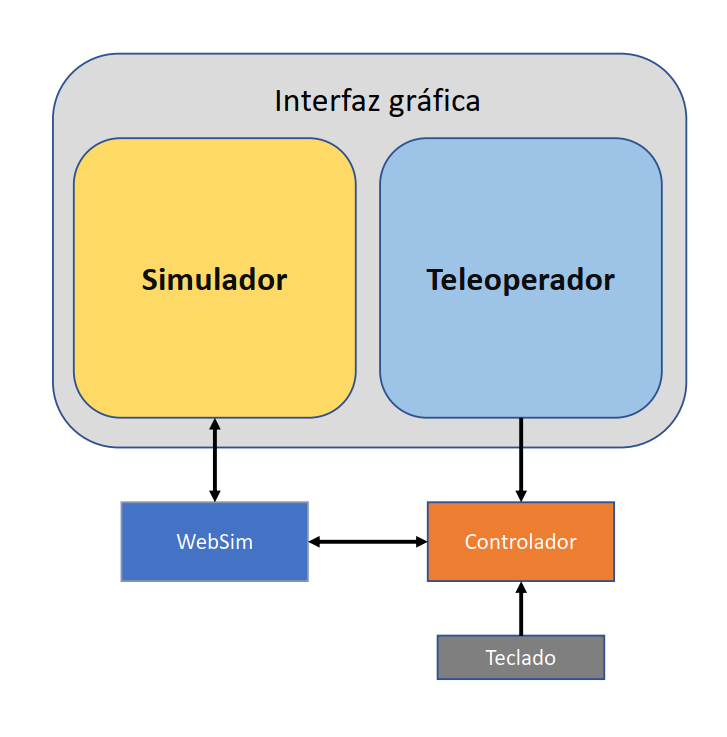
\includegraphics[scale=0.5]{img/arquitecturaTeleoperador.png}
    \caption{Arquitectura de la aplicación teleoperadores} 
    \label{fig:arq_teleop}
\end{figure}

Siendo el bloque teleoperador la interfaz creada en \textit{HTML} (\textit{listing} \ref{lst:teleop}). Se envía un evento cuando se pulsa uno de los botones del teleoperador o del teclado, que mediante un controlador se comunica con \textit{WebSim} tanto como para obtener las velocidades del robot como para enviarle las nuevas originadas por el evento, siempre usando los interfaces de programación para sensores y actuadores ofrecidos por el simulador.

Como ejemplo ilustrativo, a continuación se detalla el código del evento que inicializa el robot, los eventos que genera pulsar el teclado y los botones de la interfaz gráfica.

\begin{lstlisting}[language=javascript,label=list:traduccion]
  document.addEventListener('robot-loaded', (evt)=>{
    localRobot = evt.detail;
    console.log(localRobot);
    document.addEventListener("keydown", keypressHandler, false);
    document.addEventListener("keyup", keyupHandler, false);
    $("#speed").click(()=>{
      speed();
    });
    $("#brake").click(()=>{
      brake();
    });
    $("#left").click(()=>{
      left();
    });
    $("#right").click(()=>{
      right();
    });
    $("#up").click(()=>{
      up();
    });
    $("#down").click(()=>{
      down();
    });
    $("#takeOff").click(()=>{
      takeOff();
    });
    $("#land").click(()=>{
      land();
    });
  });
\end{lstlisting}

Las funciones llamadas cuando se pulsa el teclado comandan una velocidad fija mientras se esté pulsando: 

\begin{lstlisting}[language=javascript,label=list:teclado]
function keypressHandler(evt){
  if (evt.key == "i"){
    localRobot.setV(0.9);
  }else if(evt.key == "l"){
    localRobot.setW(-0.2);
  }else if(evt.key == "j"){
    localRobot.setW(0.2);
  }else if(evt.key == "k"){
    localRobot.setV(-0.9);
  }else if(evt.key == "u"){
    localRobot.setL(0.9);
  }else if(evt.key == "h"){
    localRobot.setL(-0.9);
  }
}
\end{lstlisting}

Cuando se pulsa alguno de los botones de la interfaz gráfica el comportamiento es diferente que pulsando el teclado: 
\begin{itemize}
    \item Flecha hacia arriba: se obtiene la velocidad lineal del robot y se incrementa.
    \begin{lstlisting}[language=javascript,label=list:speed]
    function speed(){
      let velocity = localRobot.getV()
      localRobot.setV(velocity + 0.2);
    }
    \end{lstlisting}
    \item Flecha hacia abajo: se obtiene la velocidad lineal del robot y se reduce. 
    \begin{lstlisting}[language=javascript,label=list:brake]
   function brake(){
      let velocity = localRobot.getV()
      localRobot.setV(velocity - 0.2);
    }
    \end{lstlisting}
    \item Flechas laterales: se obtiene la velocidad angular del robot y, si es distinta de 0, se le comanda una velocidad en el sentido pulsado. 
    \begin{lstlisting}[language=javascript,label=list:right]
   function right(){
      let rotation = localRobot.getW()
      if(rotation>0){
        localRobot.setW(0);
      }else{
        localRobot.setW(-0.2);
      }
    }
    function left(){
      let rotation = localRobot.getW()
      if(rotation<0){
        localRobot.setW(0);
      }else{
        localRobot.setW(0.2);
      }
    }
    \end{lstlisting}
    \item Botón de ascenso/descenso: se obtiene la velocidad vertical y se incrementa/disminuye.
    \begin{lstlisting}[language=javascript,label=list:up]
        function up(){
          let velocity = localRobot.getL()
          localRobot.setL(velocity + 0.2);
        }
        function down(){
          let velocity = localRobot.getL()
          localRobot.setL(velocity - 0.2);
        }

    \end{lstlisting}
    \end{itemize}

\subsection{WebSim y sus ficheros de configuración}

Se ha mejorado el código de \textit{WebSim} para que acepte sus ficheros de configuración en los que se especifica el escenario simulado, sus elementos, el robot elegido, distintos parámetros, etc. Esto da mucha flexibilidad al uso del simulador, qued deja de tener estos elementos directamente en el código fuente. 

Estos archivos se han creado en \textit{JSON} y se ha programado un \textit{script} (\textit{listing} \ref{list:conf}) para cargar cada fichero de configuración. Para ello se crea una variable en el \textit{index.html} del editor (\textit{listing} \ref{list:variable}) con la ruta en la que esté ubicado y el \textit{script} abre el fichero y recorre el \textit{JSON} para dar al escenario los valores establecidos.
Esta funcionalidad se ha probado y validado satisfactoriamente con los teleoperadores creados. De modo que además de mejorar el simulador para que los acepte, se han creado varios ficheros de configuración concretos como ejemplo con los diferentes \textit{robots} soportados y varios escenarios distintos. 

En los ficheros creados se pueden configurar aspectos como el modelo del robot cargado, su posición y rotación, la posición de la cámara a bordo del robot, la textura de cielo y de suelo que debe cargar o los elementos que queramos añadir en el escenario. 
\begin{lstlisting}[language=JavaScript,caption=\textit{script} que carga los ficheros de configuración,label={list:conf}]
  loadJSON(function(response) {
    var config = JSON.parse(response);
    var sceneEl = document.querySelector('a-scene');
    var robot = sceneEl.querySelector('#a-pibot');
    robot.setAttribute('gltf-model',config.robot.model);
    robot.setAttribute('scale',config.robot.scale);
    robot.setAttribute('position',config.robot.position);
    robot.setAttribute('rotation',config.robot.rotation);
    sceneEl.systems.physics.driver.world.gravity.y = config.gravity;
    sceneEl.querySelector('#ground').setAttribute('src',config.ground);
    sceneEl.querySelector('#sky').setAttribute('src',config.sky);
    sceneEl.querySelector('#ground').setAttribute('src',config.ground);
    sceneEl.querySelector('#secondaryCamera').setAttribute('position',config.secondaryCamera);
    sceneEl.querySelector('#cameraRobot').setAttribute('position',config.cameraRobot);
    if(config.objects.length>0){
      setObjects(config.objects,sceneEl);
  }
});
function setObjects(object,scene){
  for (let i in object){
    let keys = Object.keys(object[i]);
    var element = document.createElement(object[i][keys[0]]);
    for (let j = 1; j < keys.length; j++) {
      let attribute = object[i][keys[j]];
      element.setAttribute(keys[j],attribute);
    }
    scene.appendChild(element);
  }
}
\end{lstlisting}

\begin{lstlisting}[language=html,caption=variable en \textit{HTML} para indicar la ruta del fichero de configuración,label={list:variable}]
    <script>var config_file = '../assets/config/config_follow_line.json';</script>
\end{lstlisting}

\begin{lstlisting}[language=json]
  {
  "robot": {
    "model":"../assets/models/drone.gltf",
    "scale": "0.5 0.5 0.5",
    "position":"12 0 25",
    "rotation": "0 320 0"
   },
  "gravity": 0,
  "ground": "../assets/textures/escenarioLiso.png",
  "sky": "../assets/textures/sky.png",
  "secondaryCamera": "0 0 0",
  "cameraRobot":"0 0.03 -0.01",
  "objects":[{
      "type": "a-sphere",
      "position" : "12 1 15",
      "color": "#FF0000"
      }]
}
\end{lstlisting}

En este ejemplo se configura el escenario para que cargue el modelo del \textit{drone}, con el tamaño indicado en \textit{size}, la posición y rotación que aparece en \textit{position} y \textit{rotation}. En el valor \textit{gravity} se indica que el escenario no tenga gravedad, se carga la textura que posee el campo \textit{ground} como suelo del mundo y, por último, la posición de las cámaras es la ubicada en \textit{secondaryCamera} y \textit{cameraRobot}. Además, en \textit{objects} se pueden añadir todos los objetos deseados a la escena. En este ejemplo se añade al escenario una pelota de color rojo en la posición indicada.


\section{Nuevos ejercicios individuales}
\label{sec:escenarios}

Se han incorporado nuevos escenarios a \textit{WebSim} que dan la posibilidad de realizar nuevos ejercicios y mejorar los ya disponibles. En esta sección se explicarán los nuevos ejercicios desarrollados con un solo \textit{robot} en escena y sus soluciones en \textit{Scratch}.

\subsection{Sigue-líneas visión}
    Este ejercicio consiste en seguir una línea blanca sobre fondo negro haciendo uso de la cámara del \textit{robot}, que recoge las imágenes y las filtra para poder seguirla.
    
    Se ha mejorado el escenario cambiando la textura del suelo a una creada con la trazada del circuito de Interlagos de Fórmula 1. Se ha realizado con un programa de diseño gráfico (\textit{Photoshop}) y, debido a su peso computacional, se ha reducido posteriormente su tamaño para aliviar los tiempos de carga. 
    
    \begin{figure}[H]
    \centering
    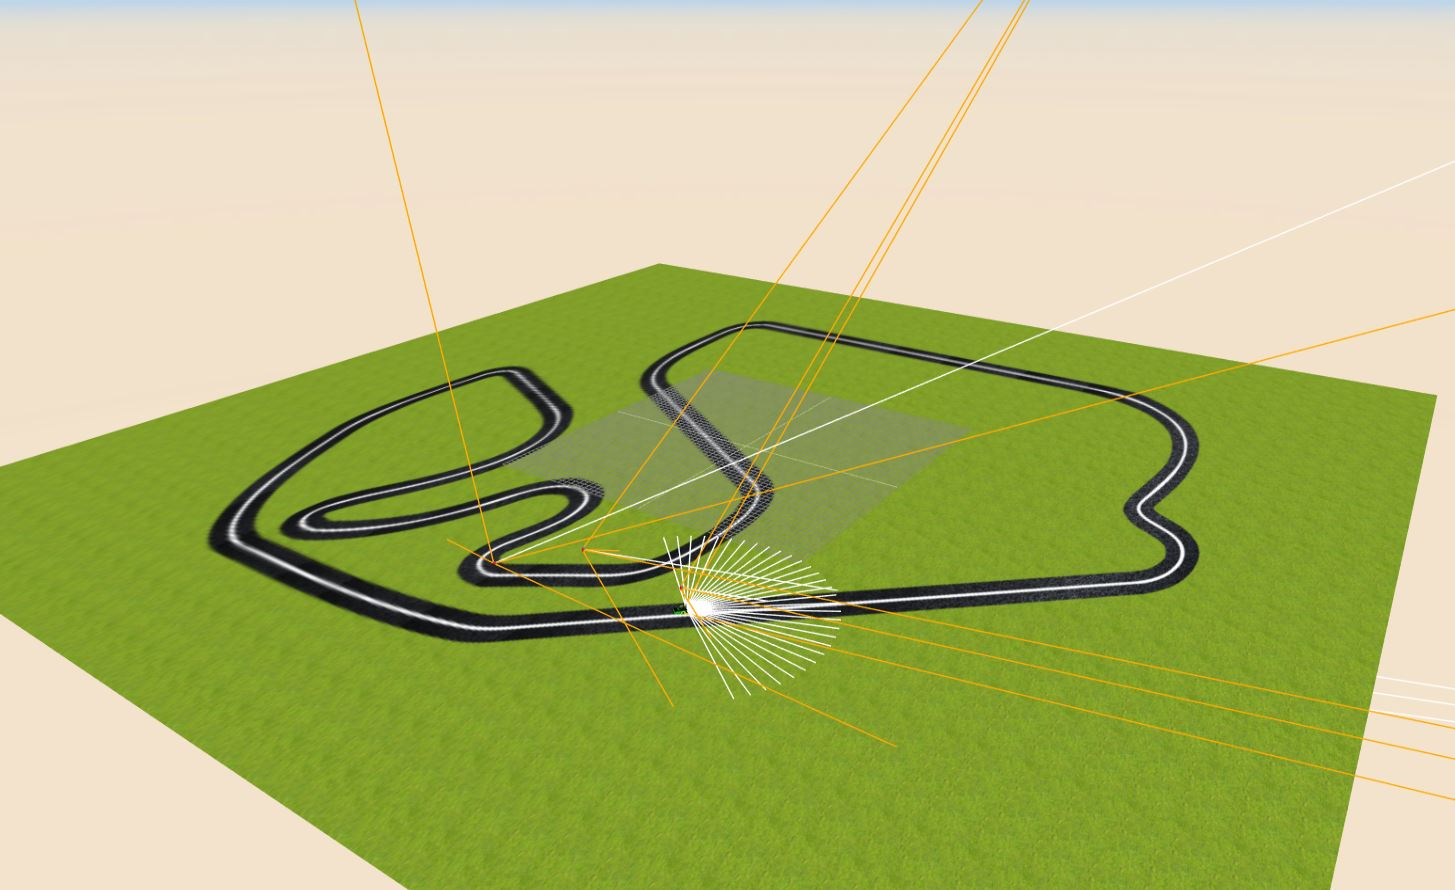
\includegraphics[scale=0.4]{img/pibot_vision.JPG}
    \caption{Escenario para el ejercicio \textit{piBot} sigue-líneas con cámara} \label{fig:siguelineavision}
    \end{figure}
    
        \begin{figure}[H]
    \centering
    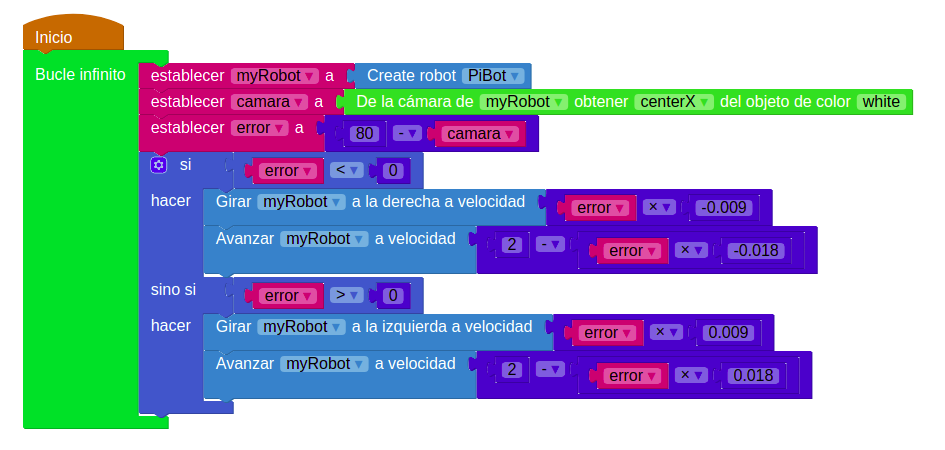
\includegraphics[scale=0.5]{img/siguelineasvisioncodigo.png}
    \caption{Solución en \textit{Scratch} para el ejercicio sigue-líneas visión} 
    \label{fig:visionSolution}
    \end{figure}
    
    En esta solución\footnote{\url{https://youtu.be/fRq__W_BETk}} se comanda velocidad lineal al robot y utiliza el bloque que obtiene el centro del eje X de los objetos blancos. Según el valor obtenido, se gira el \textit{robot} en un sentido u otro.
    
\subsection{Sigue-líneas infrarrojos}
     Este ejercicio consiste en seguir una línea negra sobre fondo blanco haciendo uso de los sensores infrarrojos del \textit{robot}. 
     
    Tiene un recorrido similar a sigue-líneas visión, pero con fondo blanco y recorrido negro para facilitar la implementación de código en el robot real y que no haya que realizar modificaciones. Para que funcionara correctamente ha sido necesario añadir el color blanco a \textit{undestandedColors} para realizar el filtro y poder pasar ``\textit{white}'' como atributo a la función \textit{getObjectColor()}.
    
    \begin{figure}[H]
    \centering
    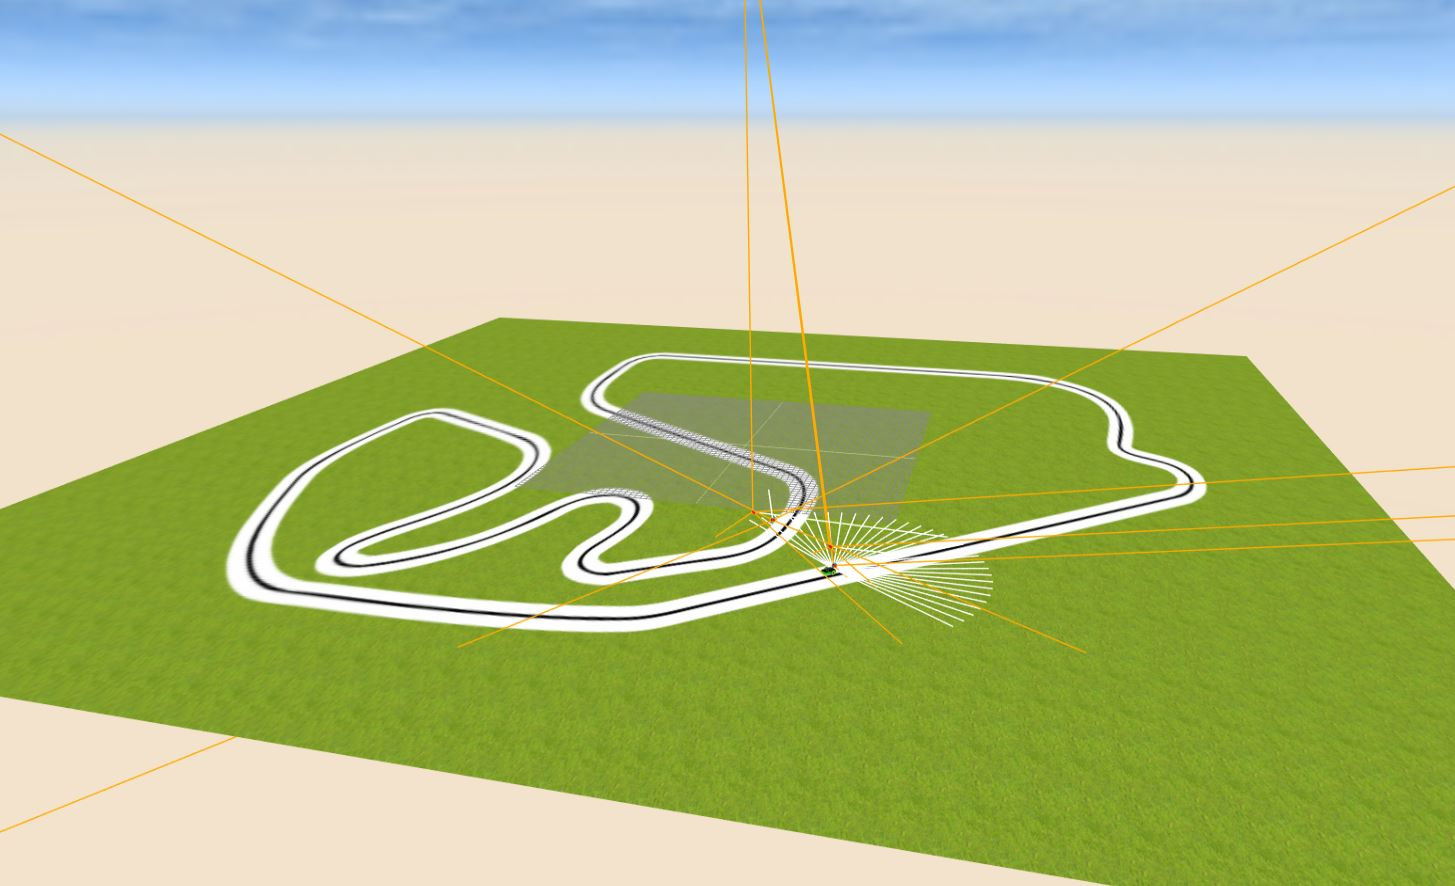
\includegraphics[scale=0.35]{img/siguelineas_ir.JPG}
    \caption{Escenario para el ejercicio para el  \textit{robot piBot} sigue-líneas infrarrojo} \label{fig:siguelineasIR}
    \end{figure}
    
           \begin{figure}[H]
    \centering
    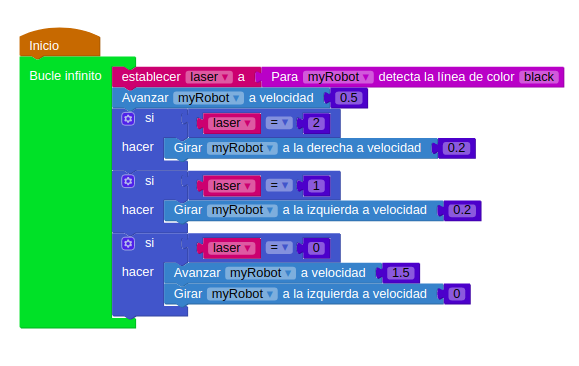
\includegraphics[scale=0.5]{img/siguelineaIRcodigo.png}
    \caption{Solución en \textit{Scratch} para el ejercicio sigue-líneas infrarrojos} 
    \label{fig:irSolution}
    \end{figure}
    
    En esta solución\footnote{\url{https://youtu.be/d4HETtPmahA}} se comanda una velocidad lineal y se obtienen los valores de los sensores infrarrojos del \textit{robot} y se comanda una velocidad angular en función de donde detecte la línea.
    
\subsection{Choca-gira}
\label{subsec:chocagira}
En este ejercicio hay programar al \textit{robot} para que avance recto mientras no haya obstáculos haciendo uso del sensor de ultra-sonidos. Si encuentra un obstáculo, tiene que detenerse, retroceder un poco, girar un ángulo aleatorio y reemprender la marcha.

Escenario creado en \textit{Blender} con un aspecto similar a su análogo en el simulador \textit{Gazebo}. Para ello se han adaptado la mayor parte de las estructuras que dispone el escenario original para su integración en \textit{WebSim}. 

    \begin{figure}[H]
    \centering
    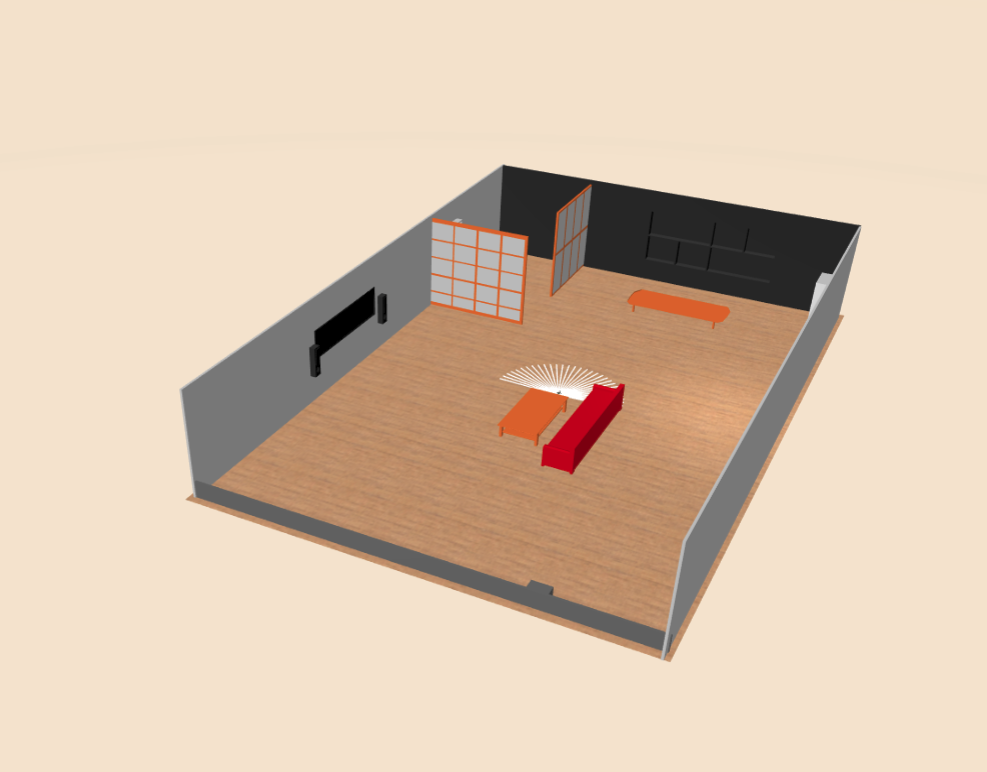
\includegraphics[scale=0.3]{img/bump&go.png}
    \caption{Escenario para el ejercicio choca-gira} \label{fig:chocagira}
    \end{figure}
    \begin{figure}[H]
    \centering
    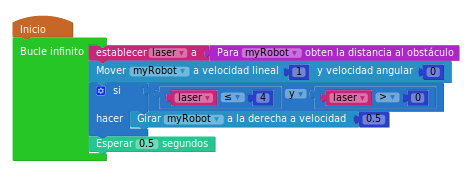
\includegraphics[scale=0.5]{img/chocagiracodigo.png}
    \caption{Solución en \textit{Scratch} para el ejercicio choca-gira} 
    \label{fig:chocagiraSolution}
    \end{figure}
    En esta solución\footnote{\url{https://youtu.be/lXL3lTbgp_E}} se obtienen los valores del sensor de ultra-sonidos y se comanda una velocidad lineal. Si encuentra un obstáculo se gira a la derecha durante 0.5 segundos.
    
\subsection{Sigue-pelota}
\label{subsec:pelota}

Este ejercicio consiste en seguir una pelota en movimiento. Hay que emplear las imágenes obtenidas por el \textit{robot} y programar la lógica de control que permita seguir la pelota.

Se ha realizado dos escenarios distintos, uno para \textit{PiBot} y otro para \textit{drone}.
Ambos disponen de una pelota de color rojo, que debe ser seguida usando la cámara del \textit{robot}, a la que se le ha dado movimiento a través de primitivas de \textit{A-Frame}. En la figura \ref{fig:secuenciaDrone} se puede ver una secuencia con la animación de una pelota y en el siguiente código se muestra el archivo de configuración de este ejercicio, que incluye esa animación de \textit{A-Frame}:

\begin{lstlisting}[language=json]
{
  "robot": {
    "model":"../assets/models/drone_animation.gltf",
    "scale": "0.5 0.5 0.5",
    "position":"12 1 25",
    "rotation": "0 50 0"
  },
  "gravity": 0,
  "ground": "../assets/textures/escenarioLiso.png",
  "sky": "../assets/textures/sky.png",
  "secondaryCamera": "4 20 30",
  "cameraRobot":"0 0.03 -0.01",
  "objects":[{
      "type": "a-sphere",
      "id":"redBall",
      "position": "4 15 20",
      "color": "#FF0000",
      "radius": "1.5",
      "animation":"property: position; from: 4 15 20 ;to: 0 15 -20; 
      dir: alternate; dur: 10000; loop: true",
      "animation__2":"property: position; from: 0 15 -20 ;to: 0 2 -20 ; delay: 10000; 
      dir: alternate; dur: 10000; loop: true",
      "animation__3":"property: position; from: 0 2 -20 ;to: 4 2 20 ; delay: 20000; 
      dir: alternate; dur: 10000; loop: true",
      "animation__4":"property: position; from: 4 2 20 ;to: 4 15 20; delay: 30000; 
      dir: alternate; dur: 10000; loop: true",
      "animation__5":"property: position; from: 4 15 20 ;to: -10 15 10; delay: 40000; 
      dir: alternate; dur: 10000; loop: true",
      "animation__6":"property: position; from: -10 15 10 ;to: 20 8 -30; delay: 50000; 
      dir: alternate; dur: 10000; loop: true"
      }]
}
\end{lstlisting}

Haciendo especial mención al campo \textit{objects}, en el que se crea una pelota roja con la animación indicada en todos los campos \textit{animation} y genera el siguiente elemento en \textit{HTML}:

\begin{lstlisting}[language=html]
<a-sphere id="redBall" position="12 1 25" color="#FF0000" radius="1.5" 
animation="property: position; from: 4 15 20 ;to: 0 15 -20; 
dir: alternate; dur: 10000; loop: true"
animation__2="property: position; from: 0 15 -20 ;to: 0 2 -20 ; delay: 10000; 
dir: alternate; dur: 10000; loop: true"
animation__3="property: position; from: 0 2 -20 ;to: 4 2 20 ; delay: 20000; 
dir: alternate; dur: 10000; loop: true" 
animation__4="property: position; from: 4 2 20 ;to: 4 15 20; delay: 30000; 
dir: alternate; dur: 10000; loop: true"
animation__5= "property: position; from: 4 15 20 ;to: -10 15 10; delay: 40000;
dir: alternate; dur: 10000; loop: true"
animation__6="property: position; from: -10 15 10 ;to: 20 8 -30; delay: 50000; 
dir: alternate; dur: 10000; loop: true">
</a-sphere>
\end{lstlisting}

\begin{figure}[H]

\begin{subfigure}[t]{0.2\textwidth}
  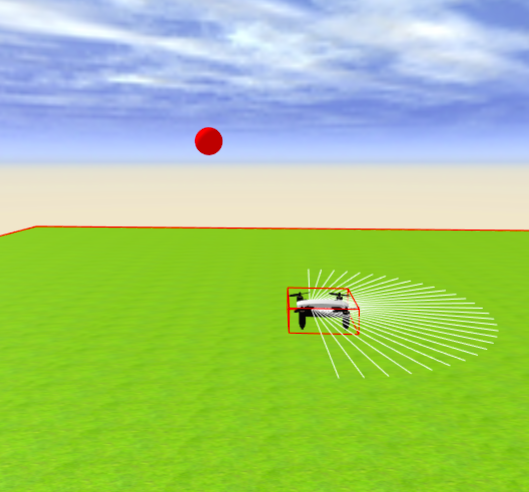
\includegraphics[width=4cm, height=4cm]{img/followBallTello2.png}
\label{fig:figure2_2}
\end{subfigure}\hfill
\begin{subfigure}[t]{0.2\textwidth}
    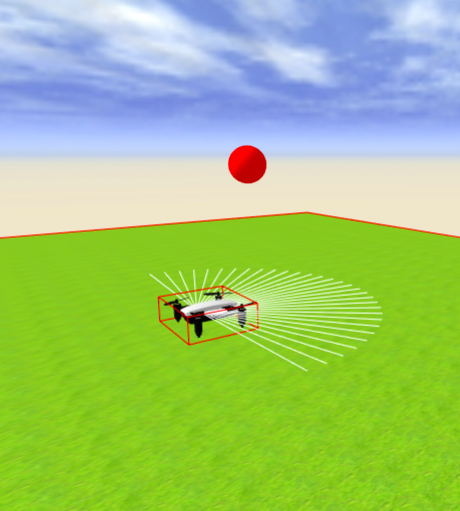
\includegraphics[width=4cm, height=4cm]{img/followBallTello3.png}
\label{fig:figure2_3}
\end{subfigure}\hfill
\begin{subfigure}[t]{0.2\textwidth}
    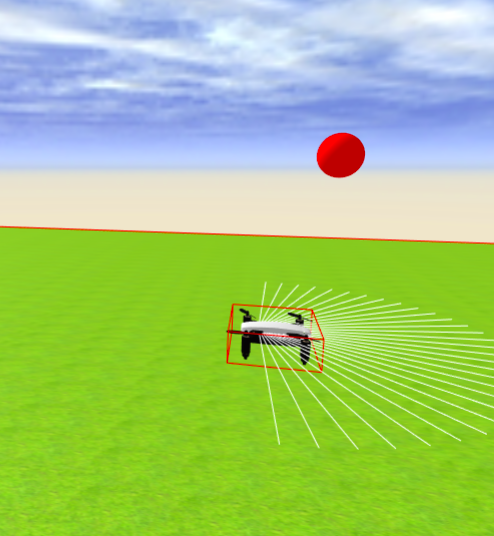
\includegraphics[width=4cm, height=4cm]{img/followBallTello4.png}
\label{fig:figure2_4}
\end{subfigure}

\begin{subfigure}[t]{0.2\textwidth}
    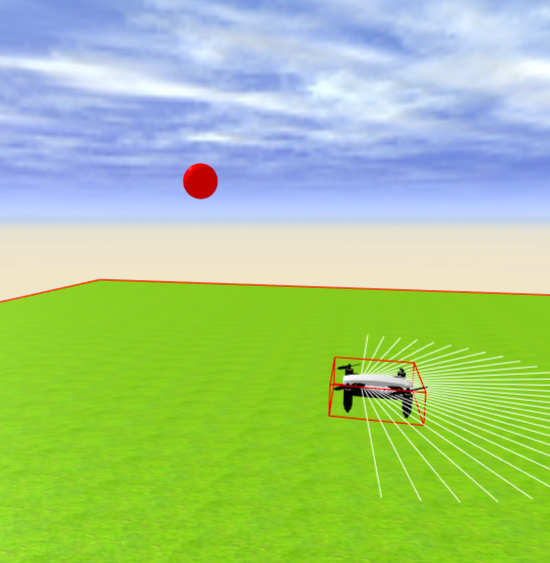
\includegraphics[width=4cm, height=4cm]{img/followBallTello6.png}
\label{fig:figure2_6}
\end{subfigure}\hfill
\begin{subfigure}[t]{0.2\textwidth}
    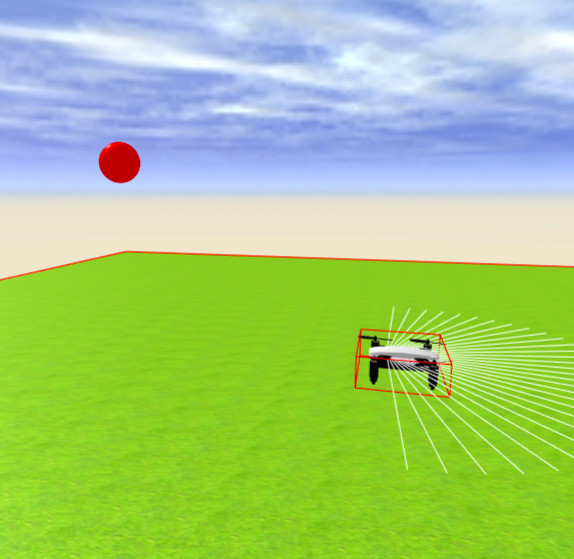
\includegraphics[width=4cm, height=4cm]{img/followBallTello7.png}
\label{fig:figure2_7}
\end{subfigure}\hfill
\begin{subfigure}[t]{0.2\textwidth}
    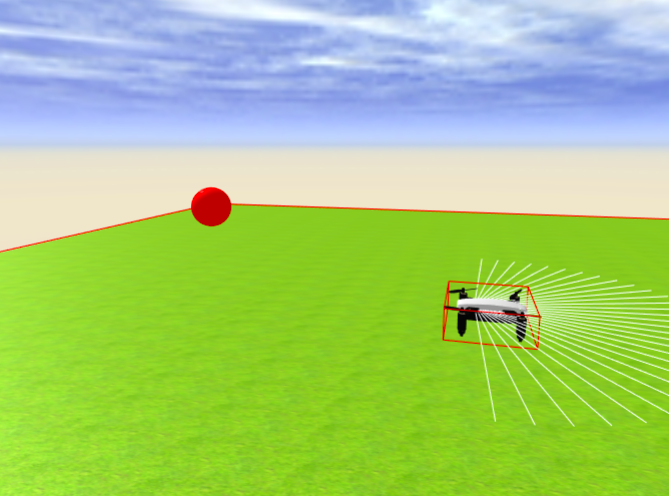
\includegraphics[width=4cm, height=4cm]{img/followBallTello8.png}
\label{fig:figure2_8}
\end{subfigure}

\caption{Secuencia de la animación de una pelota para el ejercicio \textit{drone} sigue-pelota}
\label{fig:secuenciaDrone}
\end{figure}

    \begin{figure}[H]
    \centering
    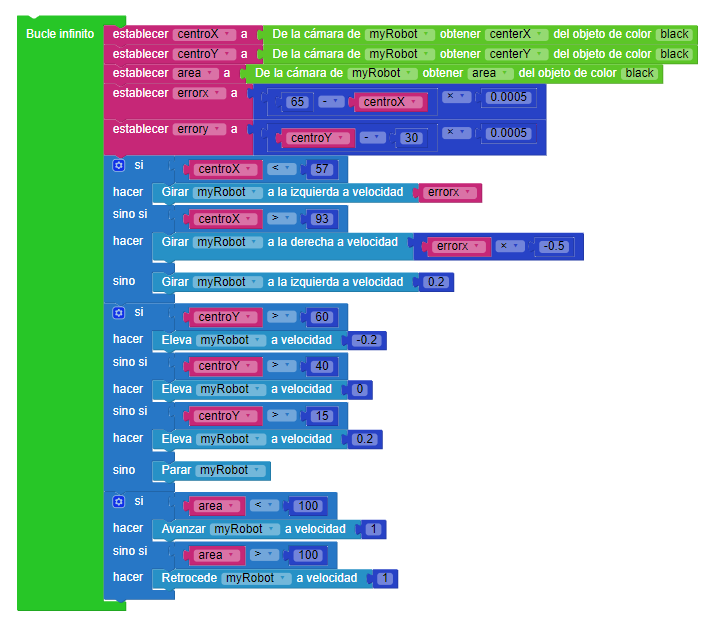
\includegraphics[scale=0.5]{img/siguepelotacodigo.png}
    \caption{Solución en \textit{Scratch} para el ejercicio sigue pelota drone} 
    \label{fig:pelotaSolution}
    \end{figure}
    La solución de este ejercicio\footnote{\url{https://youtu.be/XQrNaWxRg7U}} se ha realizado obteniendo toda la información que aporta la cámara, tanto la posición del objeto en el eje X e Y como su área. Según los valores obtenidos se comandan distintas velocidades angulares y lineales. 
\subsection{Atraviesa-bosque}
\label{subsec:atraviesabosque}
Ejercicio basado en atravesar un pasillo con diversos objetos que hay que esquivar. El sensor necesario es el infrarrojos para detectar en que posición se encuentra cada uno de los obstáculos. El escenario y los obstáculos se han creado con primitivas de \textit{A-Frame}.

    \begin{figure}[H]
    \centering
    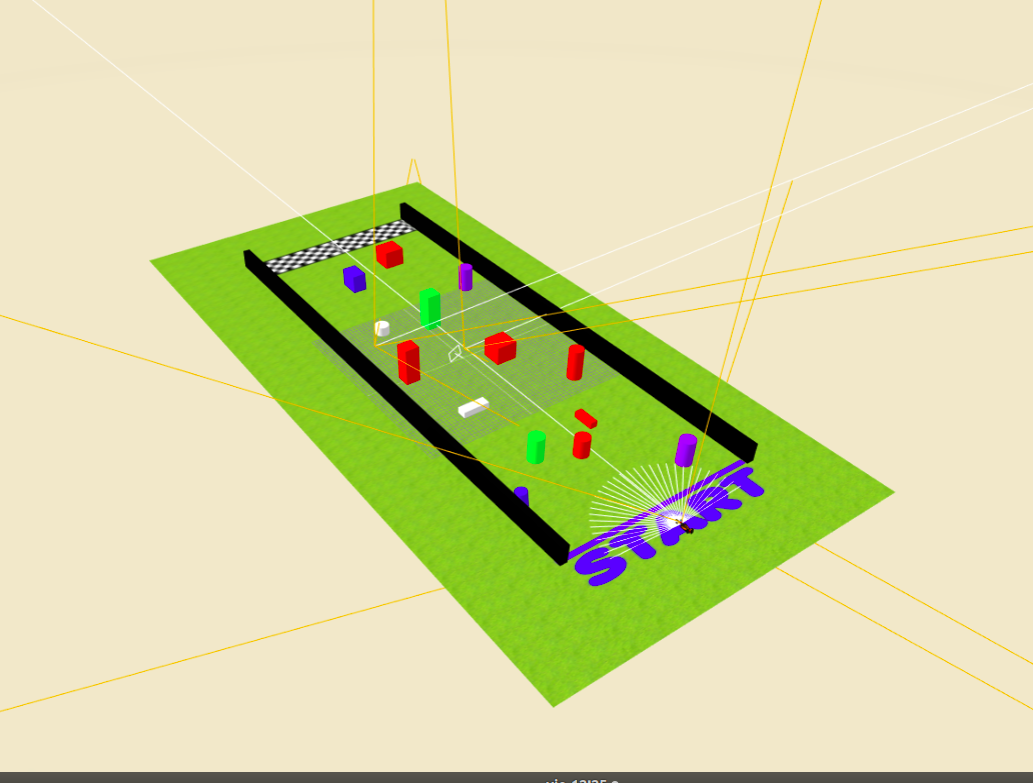
\includegraphics[scale=0.4]{img/atraviesabosque-indiv.png}
    \caption{Escenario para el ejercicio atraviesa bosque} 
    \label{fig:atraviesaBosqueind}
    \end{figure}

    \begin{figure}[H]
    \centering
    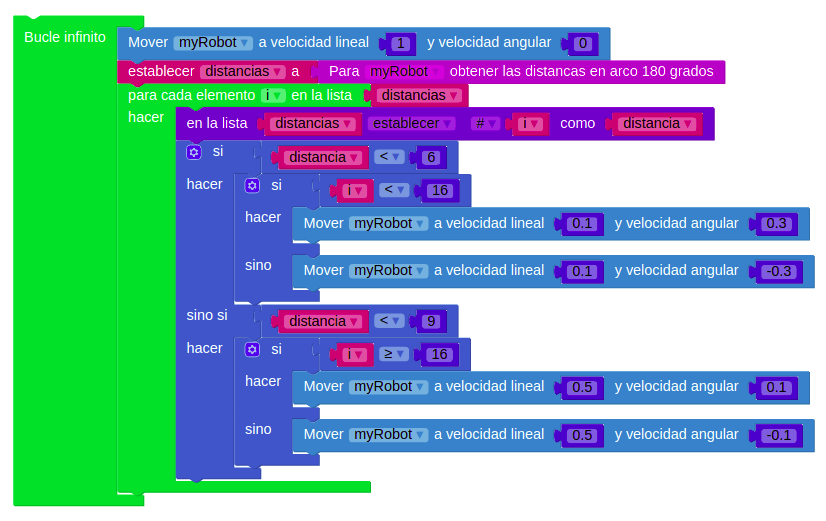
\includegraphics[scale=0.3]{img/atraviesaBosqueCodigo.png}
    \caption{Solución en \textit{Scratch} para el ejercicio atraviesa bosque} 
    \label{fig:bosqueSolution}
    \end{figure}
    
    En esta solución\footnote{\url{https://youtu.be/z3n47wWHDFc}} se obtienen todos los valores que devuelve el sensor de ultra-sonidos y, según donde detecte el obstáculo, gira en un sentido u otro.

\subsection{Cuadrado con drone}
Este ejercicio consiste en comandar velocidades al \textit{drone} para dibujar un cuadrado con el movimiento del \textit{robot}.

    \begin{figure}[H]
        \centering
        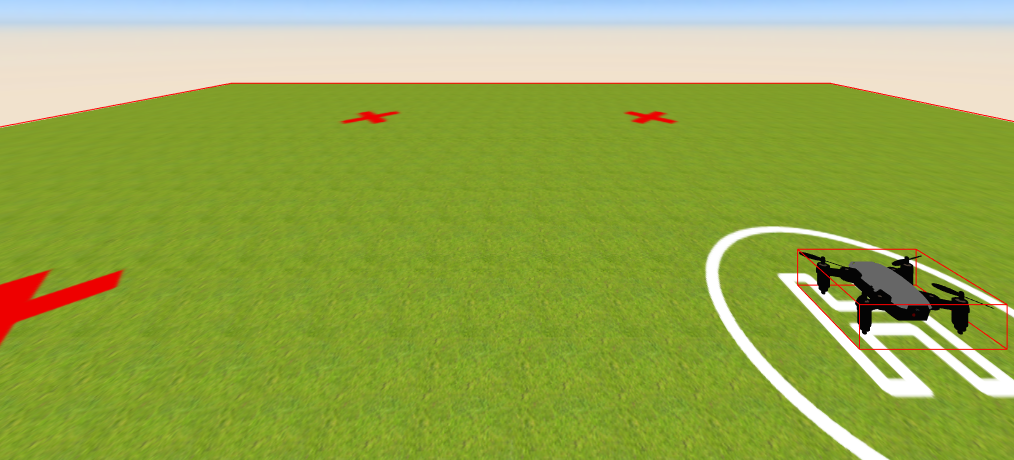
\includegraphics[scale=0.4]{img/cuadradoDrone.png}
        \caption{Escenario de WebSim para el ejercicio drone cuadrado} 
        \label{fig:droneCuadrado}
    \end{figure}

    \begin{figure}[H]
    \centering
    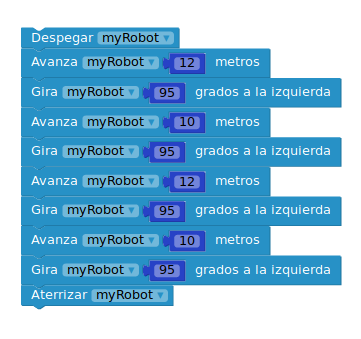
\includegraphics[scale=0.4]{img/tellocuadradocodigo.png}
    \caption{Solución en \textit{Scratch} para el ejercicio cuadrado drone} 
    \label{fig:cuadradoSolution}
    \end{figure}
    Su solución\footnote{\url{https://www.youtube.com/watch?v=XjQNhNCkOJA}} consiste en avanzar los metros necesarios para llegar a la cruz y, cuando se ha completado, girar 90 grados aproximadamente para así ``dibujar'' un cuadrado repitiendo este proceso.
    
\section{Ejercicios competitivos}
\label{sec:competitive}
Uno de los objetivos de este proyecto era añadir ejercicios competitivos a \textit{Kibotics} sobre el simulador \textit{WebSim}. Se hace especial mención a ellos debido a que son completamente diferentes al resto de los ya creados. Este tipo de ejercicios aumenta el valor de la plataforma ya que da la posibilidad de programar dos robots y ponerlos a funcionar en el mismo escenario simultáneamente, pudiendo entender la programación como un juego en el que se premia al que aporte la mejor solución.

\subsection{Arquitectura de cómputo}
\label{subsec:arquitectura}
En este tipo de ejercicios hay dos robots en una misma escena y cada uno de ellos se puede programar con un código distinto. Para su implementación e integración en \textit{Kibotics} se ha extendido el módulo \textit{brains} y se han incorporado dos aplicaciones más a \textit{WebSim}: ejercicios competitivos en \textit{Scratch} y ejercicios competitivos en \textit{JavaScript}. 
% Para su implementación se ha creado el módulo \textit{brains} en \textit{JavaScript}, que contiene el método \textit{runBrains}, que ejecuta un ``hilo'' para cada \textit{robot} existente en la escena. Además contiene los métodos \textit{stopBrain} y \textit{resumeBrain} que paran y reanudan el cerebro del robot correspondiente. 

Se ha comenzado creando la aplicación llamada \textit{competitive-JavaScript} debido a la facilidad para probar código y hacer pruebas en el entorno. Para ello se ha cambiado la interfaz del editor de código fuente, añadiendo botones para cada uno de los robots (figura \ref{fig:javascript_competitivo}) y añadido funcionalidad a cada botón para guardar el código de cada robot o mostrar el código en caso de tener uno guardado. 

    \begin{figure}[H]
        \centering            
        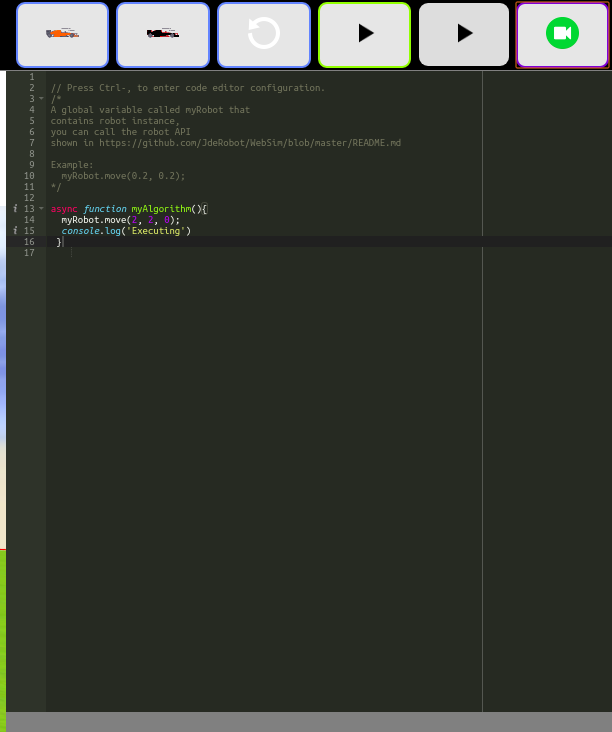
\includegraphics[scale=0.30]{img/competitiveEditorJavascript.png}
        \caption{Editor de \textit{JavaScript} para ejercicios competitivos}
        \label{fig:javascript_competitivo}
    \end{figure}
    
Cada uno de los botones tiene la funcionalidad de guardar el código escrito en el editor y, si se pulsa el botón del robot que no se está editando, se guarda el código y se carga el del otro robot en caso de que ya haya uno guardado. Si no hay ninguno se carga un editor vacío. 

\begin{lstlisting}[language=javascript]
var editFirst = true;
var editSecond = false;
var codeFirst = null;
var codeSecond = null;
  $('#firstRobot').click(()=>{
    if(editFirst){
      codeFirst = editor.getCode();
    }
    if(editSecond){
      codeSecond = editor.getCode();
      editSecond=false;
      if(codeFirst==null){
        editor.insertCode("",editor);
      }else{
        editor.insertCode(codeFirst,editor);
      }
    }
    editFirst= true;
  });
\end{lstlisting}

Cuando se pulsa el botón de ejecutar código, se ejecuta el método \textit{runBrain} del módulo \textit{brains} obteniendo previamente el código del robot que se esté editando.
\begin{lstlisting}[language=javascript]
  $("#runbtn").click(()=>{
     if (editFirst) {
       codeFirst = editor.getCode();
     } else {
       codeSecond = editor.getCode();
     }
    if (brains.threadExists(editorRobot1)){
      if (brains.isThreadRunning(editorRobot1)){
        brains.stopBrain(editorRobot1);
        brains.stopBrain(editorRobot2);
      }else{
        brains.resumeBrain(editorRobot1,codeFirst);
        brains.resumeBrain(editorRobot2,codeSecond);
      }
    }else{
      brains.runBrain(editorRobot1,codeFirst);
      brains.runBrain(editorRobot2,codeSecond);
    }
  });
\end{lstlisting}


La aplicación \textit{web} \textit{competitive-Scratch} se ha realizado de  manera similar, con la diferencia de que en este caso es necesario guardar el código de los bloques en \textit{XML} y su traducción en \textit{JavaScript}. Para realizarlo de forma limpia se ha creado un objeto que contiene un \textit{boolean} y dos cadenas de texto (\textit{listing} \ref{lst:savecode}). En el primero indica el código de qué \textit{robot} se está editando, en una cadena de texto se guarda el código \textit{XML} y en la otra su traducción en \textit{JavaScript}. Se puede ver la interfaz de este editor en la figura \ref{fig:scratch_competitivo}.
    \begin{figure}[H]
        \centering            
        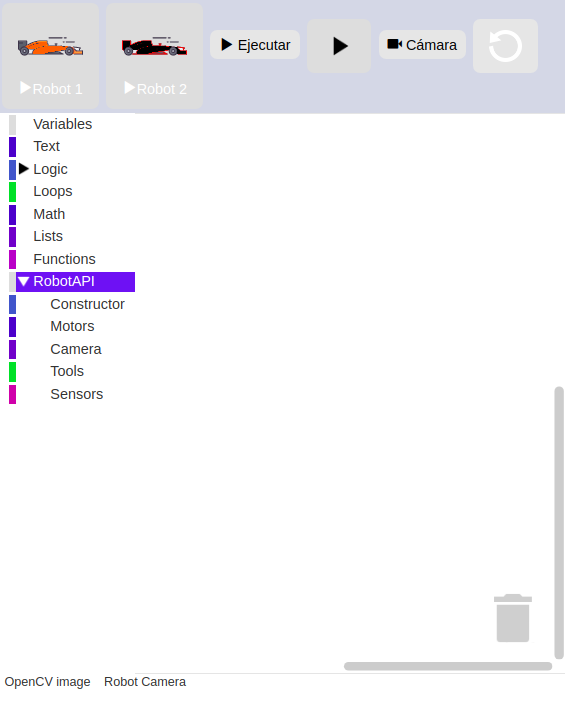
\includegraphics[scale=0.8]{img/competitivoEditorScratch.png}
        \caption{Editor de \textit{Scratch} para ejercicios competitivos}
        \label{fig:scratch_competitivo}
    \end{figure}

\begin{lstlisting}[language=javascript,label=lst:savecode, caption=código \textit{JavaScript} para guardar código de un robot]
var codeFirst = {
  js:"",
  xml:null,
  edit:true
};
var codeSecond = {
  js:"",
  xml: null,
  edit: false
};
  $('#firstRobot').click(()=>{
    if(codeFirst.edit){
      codeFirst.xml = editor.storeCode(editor.ui);
      editor.ui = editor.injectCode(editor.ui, codeFirst.xml);
    }
    if(codeSecond.edit){
      codeSecond.xml = editor.storeCode(editor.ui);
      codeSecond.edit = false;
      if(codeFirst.xml == null){
        editor.ui = editor.injectCode(editor.ui, '<xml></xml>');
      } else{
        editor.ui = editor.injectCode(editor.ui, codeFirst.xml);
      }
    }
    codeFirst.edit = true;
\end{lstlisting}

\begin{lstlisting}[language=javascript,caption=código \textit{JavaScript} para ejecutar código de los robots y guardar el que se está editando]
$("#runbtn").click(()=>{
    if (codeFirst.edit) {
        codeFirst.xml = editor.storeCode(editor.ui);
        editor.ui = editor.injectCode(editor.ui,codeSecond.xml);
        codeSecond.js = editor.getCode();
        editor.ui = editor.injectCode(editor.ui,codeFirst.xml);
        codeFirst.js = editor.getCode();
    } else {
        codeSecond.xml = editor.storeCode(editor.ui);
        editor.ui = editor.injectCode(editor.ui,codeFirst.xml);
        codeFirst.js = editor.getCode();
        editor.ui = editor.injectCode(editor.ui,codeSecond.xml);
        codeSecond.js = editor.getCode();
    }
    if (brains.threadExists(editorRobot1)){
      if (brains.isThreadRunning(editorRobot1)){
        brains.stopBrain(editorRobot1);
        brains.stopBrain(editorRobot2);
      }else{
        brains.resumeBrain(editorRobot1,codeFirst.js);
        brains.resumeBrain(editorRobot2,codeSecond.js);
      }
    }else{
      brains.runBrain(editorRobot1,codeFirst.js);
      brains.runBrain(editorRobot2,codeSecond.js);
    }
  });
\end{lstlisting}

Para puntuar el comportamiento de los robots de manera justa se han incluido en estos ejercicios \textit{evaluadores automáticos}. Van a tener diferentes comportamientos en cada ejercicio, por lo que se han desarrollado de tal forma que se pueda cargar cargar un evaluador distinto para cada uno o, incluso, no cargar ninguno. \newline

Para su implementación se ha creado el módulo \textit{evaluators}, que es similar a \textit{brains}. Tiene un método \textit{runEvaluator}, que acepta como parámetro un \textit{array} con los identificadores de los \textit{robots} a los que el código del evaluador debe conectarse para poder medir la calidad y el archivo del evaluador deseado. Este fichero se recoge como variable en el \textit{index.html} (listing \ref{lst:confEvaluator}) del editor correspondiente de forma similar a los archivos de configuración:
\begin{lstlisting}[language=html,label=lst:confEvaluator]
   <script>var config_evaluator = "evaluator_follow_line.js";</script> 
\end{lstlisting}

Para llamar a \textit{runEvaluator} se comprueba que se haya pasado un fichero en el \textit{index.html} en el código que inicializa el editor correspondiente: 

\begin{lstlisting}[language=html,label=lst:checkFile]
   if(typeof config_evaluator!=="undefined"){
    evaluators.runEvaluator([editorRobot1,editorRobot2],config_evaluator);
  }
\end{lstlisting}

En el método \textit{runEvaluator} se realiza un \textit{require} (que es la forma de importar módulos en \textit{JavaScript} de manera dinámica) de ese fichero, se crea la interfaz gráfica en el método \textit{evaluator.createInterface()} y se crea un objeto en el array de \textit{brains} que se ejecuta cada 400 milisegundos por medio del método \textit{evaluators.createTimeoutEvaluator}, que se apoya en la función \textit{setTimeout} de JavaScript. 


\begin{lstlisting}[language=javascript,caption={Funciones que crean el objeto para ejecutar el evaluador periódicamente}]
evaluators.runEvaluator = (arrayRobots,config_file)=>{
   evaluator = require("../assets/evaluators/"+config_file);
   evaluator.createInterface();
   brains.threadsBrains.push({
     "id": "evaluator",
     "running": true,
     "iteration": evaluators.createTimeoutEvaluator(arrayRobots,"evaluator"),
     "codeRunning": ""
   });
}
evaluators.createTimeoutEvaluator = (arrayRobots,id)=>{
  stopTimeoutRequested = false;
  let brainIteration = setTimeout(async function iteration(){
    evaluator.setEvaluator(arrayRobots);
    if (!stopTimeoutRequested) {
        var t = setTimeout(iteration, 400);
        var threadBrain = brains.threadsBrains.find((threadBrain)=> threadBrain.id == id);
        threadBrain.iteration = t;
    }
  }, 400);
  return brainIteration;
}
\end{lstlisting}


\subsection{Atraviesa-bosque competitivo}
\label{subsec:bosquecmp}
Este ejercicio es similar al escenario con un solo robot, pero en este caso se han creado dos pasillos en lugar de uno\footnote{\url{https://www.youtube.com/watch?v=v_aMvNPtncg}}. Se han añadido distintos objetos y elementos de \textit{A-Frame} en la misma ubicación para los dos \textit{robots} para que el recorrido sea justo.

Para su evaluador se crea una barra de progreso para cada robot y un cronómetro. Cuando se empiezan a mover los robots la barra de progreso empieza a completarse y el cronómetro se inicia, para comprobar el porcentaje completado se obtiene la posición del robot y la compara con el punto de llegada.

\begin{figure}[H]
\centering           
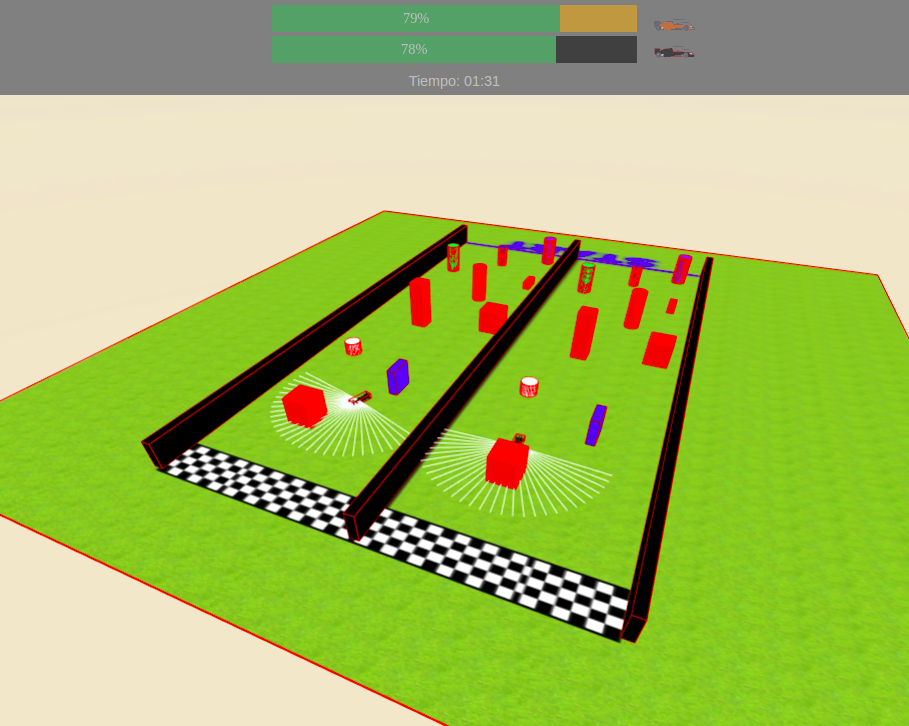
\includegraphics[scale=0.3]{img/evaluador_forest.png}
\caption{Escenario y evaluador para el ejercicio atraviesa-bosque}
\label{fig:evaluador_bosque}
\end{figure}


Las funciones necesarias para el evaluador se definen a continuación: 
\begin{itemize}
    \item Una dedicada a crear la interfaz que establece los elementos necesarios para añadir las barras de progreso, iconos, tiempo y sus atributos.
\begin{lstlisting}[language=javascript]
evaluator.createInterface= ()=>{
  var node = document.createElement("div");
  node.setAttribute("class","evaluator");
  var img1 = document.createElement("img");
  img1.setAttribute("class","carMarker");
  img1.setAttribute("src","../assets/resources/car1.svg")
  node.appendChild(img1);
  var node2 = document.createElement("div");
  node2.setAttribute("id","car1Progress");
  var node3 = document.createElement("div");
  node3.setAttribute("id","a-car1bar");
  node3.innerHTML = "0%";
  node2.appendChild(node3);
  node.appendChild(node2);
  var img2 = document.createElement("img");
  img2.setAttribute("class","carMarker");
  img2.setAttribute("src","../assets/resources/car2.svg")
  node.appendChild(img2);
  var node4 = document.createElement("div");
  node4.setAttribute("id","car2Progress");
  var node5 = document.createElement("div");
  node5.setAttribute("id","a-car2bar");
  node5.innerHTML = "0%";
  node4.appendChild(node5);
  node.appendChild(node4);
  var time = document.createElement("div");
  time.setAttribute("id","time");
  time.innerHTML="Tiempo: 00:00";
  time.style.marginTop="-87px";
  time.style.color="white";
  node.appendChild(time);
  var myiframe= document.getElementById("myIFrame");
  myiframe.insertBefore(node,myiframe.childNodes[0]);
}
\end{lstlisting}
    \item La función que se ejecuta periódicamente comprueba la velocidad de los robots y, si es mayor que 0, se inician los evaluadores, llama a una función que realiza la lógica para actualizar las barras de progreso y añadir un cronómetro al \textit{DOM}. La variable \textit{timeInit} se actualiza constantemente hasta que el usuario ejecuta su código y el \textit{robot} comienza a moverse, que se calcula el tiempo transcurrido y lo muestra en pantalla.
\begin{lstlisting}[language=javascript]
evaluator.setEvaluator = (arrayRobots) =>{
  let robot=Websim.robots.getHalAPI(arrayRobots[0]);
  if(!clock){
    timeInit = new Date();
  }
  if(robot.velocity.x>0){
    clock=true;
    var time= document.getElementById("time");
    progressBar(arrayRobots);
    var realTime = new Date(new Date() - timeInit);
    var formatTime = timeFormatter(realTime);
    time.innerHTML = "Tiempo: " + formatTime;
  }
}
\end{lstlisting}
    \item Función que calcula el porcentaje recorrido por cada uno de los \textit{robots}, modifica las barras de progreso y lo añade al \textit{DOM} para que aparezca en texto.
    
  \begin{lstlisting}[language=javascript]
function progressBar(arrayRobots){
  arrayRobots.forEach(function(robotID){
    let robot = Websim.robots.getHalAPI(robotID);
    var left=38.24 + robot.getPosition().x;
    var completed=(left*100)/78.48;
    var element = document.getElementById(robot.myRobotID+"bar");
    if((100-completed)>100){
      element.style.width = 100 + '%';
      element.innerHTML = 100 + '%';
    }else{
      element.style.width = Math.round(100-completed) + '%';
      element.innerHTML = Math.round(100-completed) + '%';
    }
  });
}
\end{lstlisting}
        \item Función que da formato al cronómetro.
\begin{lstlisting}[language=javascript]
function timeFormatter(time){
  var formatTime;
  if (time.getMinutes()<10){
    formatTime="0"+time.getMinutes();
  }else{
    formatTime=time.getMinutes();
  }
  formatTime+=":";
  if (time.getSeconds()<10){
    formatTime+="0"+time.getSeconds();
  }else{
    formatTime+=time.getSeconds();
  }
  return formatTime;
}
\end{lstlisting}
\end{itemize}

\subsection{Sigue-líneas competitivo}
\label{subsec:race}

En este ejercicio hay dos robots en el que tienen que seguir una linea de color blanco sobre fondo negro atravesando un puente en medio del circuito para que, de esta manera, ambos recorran la misma distancia\footnote{\url{https://www.youtube.com/watch?v=OaA7_wsXhk8}}.

La principal novedad del escenario es el puente creado, que permite ser cruzado mientras siguen la línea. La solución definitiva ha sido creando primitivas de \textit{A-Frame} (\textit{a-plane}) y añadiendo una textura diseñada con \textit{Photoshop} con el mismo aspecto que el resto del circuito.

El evaluador de este ejercicio es similar al de atraviesa-bosque, con la diferencia de que es necesario guardar en todo momento la posición y distancia recorrida por cada robot para calcular el porcentaje del circuito completado. 
\begin{lstlisting}[language=javascript,caption=Objeto creado para guardar posición y distancia recorrida de un robot]
var car={
    pos:{
        x:robot.getPosition().x,
        z:robot.getPosition().z
    },
    dist: 0
}
\end{lstlisting}

 \begin{lstlisting}[language=javascript,caption=Función que realiza la funcionalidad para rellenar la barra de progreso]
evaluator.setEvaluator = (arrayRobots) => {
  let robot1=Websim.robots.getHalAPI(arrayRobots[0]);
  let robot2=Websim.robots.getHalAPI(arrayRobots[1]);
  if(!clock){
    timeInit = new Date();
    car1 = {
        pos:{
                x:robot1.getPosition().x,
                z:robot1.getPosition().z
            },
            dist: 0
    };
    car2 = {
        pos:{
            x:robot2.getPosition().x,
            z:robot2.getPosition().z
        },
        dist: 0
    }
  }
  if(robot1.velocity.x>0){
    clock=true;
    var time= document.getElementById("time");
    progressBar(arrayRobots,[car1,car2]);
    var realTime = new Date(new Date() - timeInit);
    var formatTime = timeFormatter(realTime);
    time.innerHTML = "Tiempo: " + formatTime;
  }
}
\end{lstlisting}
            
\begin{figure}[H]
    \centering           
    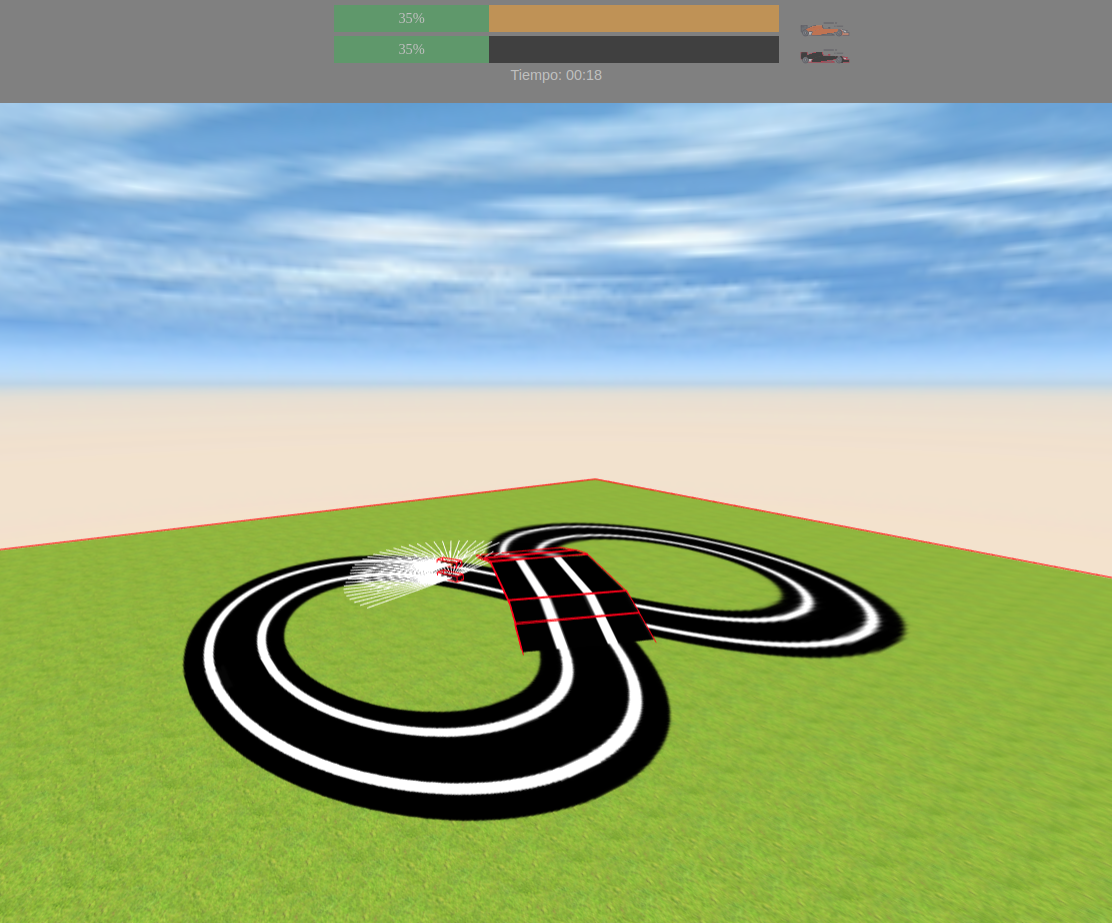
\includegraphics[scale=0.2]{img/evaluator_follow_line.png}
    \caption{Ejercicio y evaluador sigue-líneas competitivo}
    \label{fig:evaluador_siguelineas}
\end{figure}

\subsection{Gato-ratón}
\label{subsec:gatoraton}
No es estrictamente hablando un ejercicio competitivo directamente, con dos códigos de estudiantes sobre sendos robots en el mismo escenario simultáneamente. En este ejercicio hay dos robots, uno (el \textit{drone} gato) programado por el estudiante que hace el ejercicio y otro (el \textit{drone} ratón) programado por desarrolladores de la plataforma. 
En este ejercicio el usuario tiene que desarrollar su solución para que el \textit{robot} no se aleje del objetivo, el \textit{drone} ratón, que está en constante movimiento\footnote{\url{https://www.youtube.com/watch?v=xA9Emhdk_HQ}}. 


Para este ejercicio se ha creado un \textit{script} llamado \textit{agents-methods.js}, basado en \textit{brains}, para ejecutar el código del \textit{drone} ratón sin necesidad de escribir código. Es muy similar al método \textit{runBrain} con la diferencia de que el código viene de un fichero en lugar del editor. En este módulo se guarda el código en la variable \textit{agents.code} con el siguiente código: 

\begin{lstlisting}[language=javascript]
agents.getCode = (file) => {
  var request = new XMLHttpRequest();
  request.open("GET", file);
  request.onreadystatechange = function () {
    if(request.status === 200 || request.status == 0) {
        agents.code = request.responseText;
    }
  }
  request.send();
}
\end{lstlisting}

Siendo \textit{file} una variable que se inicializa en el \textit{index.html} de manera similar a los ficheros de configuración y evaluadores automáticos. 
Una vez obtenido el código se llama al método \textit{runAgent} que recoge el código e incorpora la lógica programada en el \textit{array} de \textit{robots} del módulo \textit{brains}.

\begin{lstlisting}[language=javascript]
agents.runAgent = (robotID, code) =>{
  code = 'async function myAlgorithm(){\n'+code+'\n}\nmyAlgorithm();';
  brains.threadsBrains.push({
    "id": robotID,
    "running": true,
    "iteration": brains.createTimeoutBrain(code, Websim.robots.getHalAPI(robotID), robotID),
    "codeRunning": code
  });
}
\end{lstlisting}

A la hora de ejecutar el código, se elige si el código que se ejecuta es el que hay en el agente llamando al método \textit{runAgent} del módulo \textit{agents} o el que hay en el editor con el método \textit{runBrain} del módulo \textit{brains}. \\
En el siguiente código se ejecuta en un \textit{robot} el código escrito en el editor y en otro el escrito en el agente:

\begin{lstlisting}[language=javascript]
  $("#runbtn").click(()=>{
     if (editFirst) {
       codeFirst = editor.getCode();
     } else {
       codeSecond = editor.getCode();
     }
    if (brains.threadExists(editorRobot1)){
      if (brains.isThreadRunning(editorRobot1)){
        brains.stopBrain(editorRobot1);
        brains.stopBrain(editorRobot2);
      }else{
        brains.resumeBrain(editorRobot1,codeFirst);
        agents.resumeAgent(editorRobot2,agents.code);
      }
    }else{
      brains.runBrain(editorRobot1,codeFirst);
      agents.runAgent(editorRobot2,agents.code);
    }
  });\end{lstlisting}
  
  
Para el evaluador de este ejercicio se crea un gráfico con ayuda de una librería externa de \textit{JavaScript} (\textit{JavaScript Graphics Library}\footnote{\url{http://www.jsgl.org/}}) que muestra la distancia entre \textit{drones} y el tiempo que lleva de ejecución. Se puede ver este evaluador en la figura \ref{fig:evaluador_gato_raton}. 
 En este caso, el método \textit{createInterface} realiza añade todo lo necesario al \textit{DOM} para que el gráfico sea completo y llama a la función \textit{setAxis()} para añadir los ejes y las etiquetas.
 \begin{lstlisting}[language=javascript,caption=Función que establece los ejes y etiquetas de la gráfica]
 evaluator.createInterface= ()=>{
  var node = document.createElement("div");
  node.setAttribute("id","panel");
  node.style.height="130px";
  node.style.backgroundColor="white";
  var time = document.createElement("div");
  time.setAttribute("id","time");
  time.marginLeft="50px";
  time.innerHTML="Tiempo: 00:00";
  time.style.color="black";
  time.style.textAlign="center";
  node.appendChild(time);
  var myiframe= document.getElementById("myIFrame");
  myiframe.insertBefore(node,myiframe.childNodes[0]);
  myPanel = new jsgl.Panel(document.getElementById("panel"));
  setAxis(myPanel);
  line = myPanel.createPolyline();
  line.getStroke().setColor('blue');
  line.getStroke().setWeight(2);
}
\end{lstlisting}

\begin{lstlisting}[language=javascript,caption=Método \textit{createInterface}]
function setAxis(myPanel){
  var axisX = myPanel.createLine();
  axisX.setStartPointXY(20,10);
  axisX.setEndPointXY(20,100);
  myPanel.addElement(axisX);
  var axisY = myPanel.createLine();
  axisY.setStartPointXY(20,100);
  axisY.setEndPointXY(500,100);
  myPanel.addElement(axisY);
  var myLabel = myPanel.createLabel();
  myLabel.setLocation(new jsgl.Vector2D(75,100));
  myLabel.setText("00:30");
  myPanel.addElement(myLabel);
  var myLabel = myPanel.createLabel();
  myLabel.setLocation(new jsgl.Vector2D(0,20));
  myLabel.setText("10");
  myPanel.addElement(myLabel);
}
\end{lstlisting}

\begin{lstlisting}[language=javascript,caption={Código JavaScript que calcula la distancia entre \textit{drones}, la representa e incorpora un cronómetro al \textit{DOM}}]
evaluator.setEvaluator = (arrayRobots) => {
  var robot1 = Websim.robots.getHalAPI(arrayRobots[0]);
  var robot2 = Websim.robots.getHalAPI(arrayRobots[1]);
  if(!clock){
    timeInit = new Date();
  }
  if(robot1.velocity.x >0 || robot2.velocity.x>0){
    clock = true;
    var time= document.getElementById("time");
    var realTime = new Date(new Date() - timeInit);
    var formatTime = timeFormatter(realTime);
    time.innerHTML = "Tiempo: " + formatTime;
    var pos1 = robot1.getPosition();
    var pos2 = robot2.getPosition();
    var dist = Math.sqrt(Math.pow(pos2.x-pos1.x,2)+Math.pow(pos2.y-pos1.y,2)+Math.pow(pos2.z-pos1.z,2));
    line.addPointXY(x,dist+10);
    x=x+0.5;
    myPanel.addElement(line);
  }
}
\end{lstlisting}
\begin{figure}[ht]
\centering           
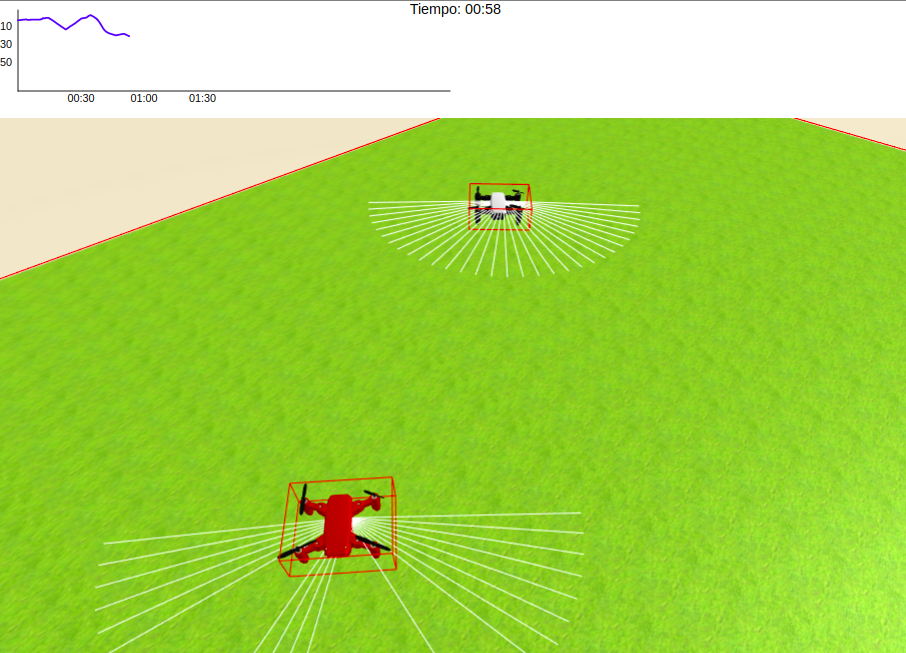
\includegraphics[scale=0.3]{img/evaluador_drone.png}
\caption{Evaluador y escenario con dos robots para ejercicio gato-ratón}
\label{fig:evaluador_gato_raton}
\end{figure}
